\originalchapter{8.05 作业11：径向问题与角动量合成}
来源为Fall 2013 Assignment 11, 2013年11月29日发布, 12月6日15时截止. 本篇纳入正式作业六题与PRACTICE六题; 后者原文明确“不提交”, 不混作有分正式考核. 以下均为\textbf{AI独立解答}. 原件建议参考外书CG表或Shankar解答, 此处自行推导, 未取得或打包外书. 题面称卷末有CG表, 实际PDF末页仅OCW声明, 不声称已核不存在的表.
\originalsection{正式第1题：自旋1的连续测量}
\begin{exercise}
在$\ket{1,m}$按$m=1,0,-1$排序, 求$L^2,L_\pm,L_x,L_y,L_z$矩阵, 验$[L_x,L_y]=\ii\hbar L_z$, 求$L_x$三本征态. 从$x+$测$z$的分布为何? 若先得$z-$再测$x$、又得$x-$再测$z$, 每步给概率.
\end{exercise}
\begin{solution}
$L^2=2\hbar^2I$, $L_z=\hbar\operatorname{diag}(1,0,-1)$,
\[
L_+=\sqrt2\hbar\begin{pmatrix}0&1&0\\0&0&1\\0&0&0\end{pmatrix},\quad L_-=L_+^\dagger,\quad
L_x=\frac\hbar{\sqrt2}\begin{pmatrix}0&1&0\\1&0&1\\0&1&0\end{pmatrix},\quad
L_y=\frac\hbar{\sqrt2}\begin{pmatrix}0&-\ii&0\\\ii&0&-\ii\\0&\ii&0\end{pmatrix}.
\]
直接乘$L_xL_y-L_yL_x$给$\ii\hbar^2\operatorname{diag}(1,0,-1)$. $x+$、$x0$、$x-$单位矢分别$(1,\sqrt2,1)/2$、$(1,0,-1)/\sqrt2$、$(1,-\sqrt2,1)/2$. $x+$测$z$结果$\hbar,0,-\hbar$概率$1/4,1/2,1/4$. 条件$z-$后测$x$仍$1/4,1/2,1/4$; 再条件$x-$后测$z$亦同. 每次理想测量条件态替换前态, 最后一组不是将之前概率再乘进去的条件概率; 若要原始束的联合链概率才相乘.
\end{solution}
\originalsection{正式第2题：氢Hamilton算符平方分解}
\begin{exercise}
将$H=p^2/(2m)-e^2/r$写为$\gamma+\sum_k(p_k+\ii\beta x_k/r)(p_k-\ii\beta x_k/r)/(2m)$, 求实$\beta,\gamma$, 证明能量下界并找饱和归一态.
\end{exercise}
\begin{solution}
令$n_k=x_k/r$. 乘积展开为$p^2+\beta^2+\ii\beta\sum[n_k,p_k]=p^2+\beta^2-2\beta\hbar/r$, 因$\nabla\cdot\boldsymbol n=2/r$. 故$\beta=me^2/\hbar=\hbar/a_0$, $\gamma=-\beta^2/(2m)=-me^4/(2\hbar^2)$. 每个乘积是$Q_k^\dagger Q_k$, $Q_k=p_k-\ii\beta n_k$, 在适当Coulomb形式域均值非负, 所以$\langle H\rangle\ge\gamma$.

饱和须$Q_k\psi=0$各$k$, 即$\partial_k\psi=-x_k\psi/(a_0r)$. 梯度平行径向, 解$\psi=C\e^{-r/a_0}$, $C=(\pi a_0^3)^{-1/2}$. 它归一且满足全部一阶方程, 达下界即基态. $e^2$沿原题Coulomb常数单位, SI要整体替为$e^2/(4\pi\epsilon_0)$.
\end{solution}
\originalsection{正式第3题：突然核电荷变化}
\begin{exercise}
氚基态电子遇瞬间$\beta$衰变, 核电荷从1变2且忽略约化质量变化. 求衰变后立刻处于He⁺基态的概率, 以及处于某个$\ell=0$态的总概率.
\end{exercise}
\begin{solution}
突然近似使电子波函数来不及变化, 投影到新态. $Z$基态$\psi_Z=\sqrt{Z^3/(\pi a_0^3)}\e^{-Zr/a_0}$, 重叠$8(Z_1Z_2)^{3/2}/(Z_1+Z_2)^3$, $Z_1=1,Z_2=2$得$16\sqrt2/27$, 概率$512/729\simeq0.702332$. 初始球对称, 新中心势角动量基完整, 只含$\ell=0$径向态, 其总概率1; 包括连续谱的$s$波, 不意味剩下约30\%都在束缚激发态. 不将中性He的双电子态误套本题单电子He⁺.
\end{solution}
\originalsection{正式第4题：有限球井与三维点势调节}
\begin{exercise}
球井$r<a$势$-V_0$、外0, $V_0=v_0^2\hbar^2/(2ma^2)$. (a)(b)求$s$波束缚阈值与方程, 记$E=-\epsilon^2\hbar^2/(2ma^2)$. (c)作图分析大$v_0$低态能量及基态首修正. (d)以$V_a=-V_0(L/a)^3$于$r<a$调节$-4\pi V_0L^3\delta^3(r)/3$, 核积分、求$a\to0$能谱行为, 由量纲解释问题.
\end{exercise}
\begin{solution}
$s$波$u(0)=0$, 内$u=A\sin(\eta r/a)$、外$B\e^{-\epsilon r/a}$, 其中$\eta^2+\epsilon^2=v_0^2$, 接续给$-\eta\cot\eta=\epsilon$. 第一正支在$\eta>\pi/2$, 故真实束缚需要$v_0>\pi/2$, 等号只是非归一阈值. 图为$\epsilon=-\eta\cot\eta$正支与半径$v_0$圆在第一象限交点. 低整数$n$、大$v_0$时$\eta_n=n\pi-\delta_n$, $\delta_n\simeq n\pi/v_0$, 所以
\[
E_n=-V_0+\frac{(n\pi)^2\hbar^2}{2ma^2}
\left(1-\frac2{v_0}+O(v_0^{-2})\right).
\]
对$n=1$首修正负, 表示有限井渗透使有效宽度增加; 相比无限壁能级降低.
\begin{center}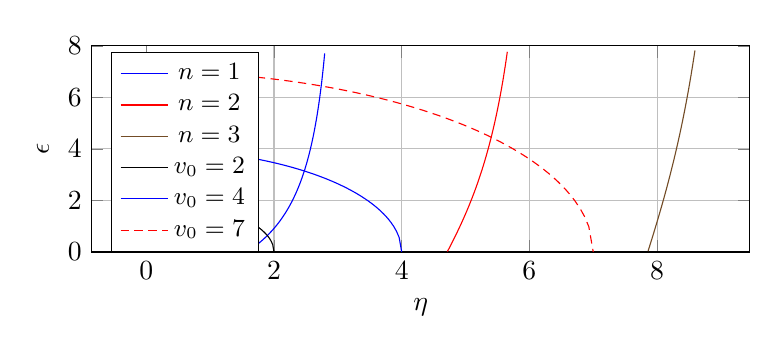
\begin{tikzpicture}
\begin{axis}[width=.82\textwidth,height=4.2cm,xlabel={$\eta$},ylabel={$\epsilon$},grid=major,legend style={font=\small},ymin=0,ymax=8,legend pos=north west]
\addplot+[mark=none] coordinates{(1.57479633,0.0062992189) (1.59042429,0.031220799) (1.60605225,0.0566463323) (1.62168022,0.0825886885) (1.63730818,0.109061271) (1.65293614,0.136078046) (1.66856411,0.16365357) (1.68419207,0.191803022) (1.69982003,0.220542238) (1.715448,0.249887745) (1.73107596,0.279856799) (1.74670392,0.310467428) (1.76233189,0.341738471) (1.77795985,0.373689628) (1.79358781,0.406341508) (1.80921578,0.439715682) (1.82484374,0.47383474) (1.8404717,0.50872235) (1.85609967,0.544403327) (1.87172763,0.580903699) (1.88735559,0.618250785) (1.90298356,0.656473275) (1.91861152,0.695601315) (1.93423948,0.735666607) (1.94986745,0.776702504) (1.96549541,0.818744122) (1.98112337,0.861828458) (1.99675134,0.905994518) (2.0123793,0.951283456) (2.02800726,0.997738725) (2.04363522,1.04540623) (2.05926319,1.09433454) (2.07489115,1.14457501) (2.09051911,1.19618207) (2.10614708,1.24921342) (2.12177504,1.30373026) (2.137403,1.35979759) (2.15303097,1.41748451) (2.16865893,1.47686453) (2.18428689,1.53801594) (2.19991486,1.6010222) (2.21554282,1.66597241) (2.23117078,1.73296172) (2.24679875,1.80209193) (2.26242671,1.87347205) (2.27805467,1.94721895) (2.29368264,2.02345809) (2.3093106,2.10232431) (2.32493856,2.18396276) (2.34056653,2.26852987) (2.35619449,2.35619449) (2.37182245,2.44713914) (2.38745042,2.54156144) (2.40307838,2.63967569) (2.41870634,2.74171468) (2.43433431,2.84793173) (2.44996227,2.95860303) (2.46559023,3.07403022) (2.4812182,3.19454348) (2.49684616,3.32050493) (2.51247412,3.45231262) (2.52810209,3.59040509) (2.54373005,3.73526669) (2.55935801,3.8874337) (2.57498598,4.04750147) (2.59061394,4.21613286) (2.6062419,4.39406804) (2.62186987,4.58213611) (2.63749783,4.78126891) (2.65312579,4.99251746) (2.66875376,5.21707161) (2.68438172,5.45628378) (2.70000968,5.71169776) (2.71563765,5.98508378) (2.73126561,6.27848162) (2.74689357,6.594254) (2.76252154,6.93515314) (2.7781495,7.30440446) (2.79377746,7.70581294)};
\addlegendentry{$n=1$}
\addplot+[mark=none] coordinates{(4.71638898,0.0188656565) (4.73201694,0.0928917841) (4.74764491,0.167452006) (4.76327287,0.242583251) (4.77890083,0.318323091) (4.7945288,0.39470981) (4.81015676,0.471782488) (4.82578472,0.549581079) (4.84141269,0.628146492) (4.85704065,0.707520682) (4.87266861,0.787746739) (4.88829658,0.868868985) (4.90392454,0.950933072) (4.9195525,1.03398609) (4.93518047,1.11807666) (4.95080843,1.2032551) (4.96643639,1.28957348) (4.98206436,1.37708582) (4.99769232,1.46584819) (5.01332028,1.55591885) (5.02894825,1.64735846) (5.04457621,1.7402302) (5.06020417,1.83459999) (5.07583214,1.93053665) (5.0914601,2.02811213) (5.10708806,2.12740173) (5.12271603,2.22848436) (5.13834399,2.33144278) (5.15397195,2.43636389) (5.16959992,2.54333903) (5.18522788,2.65246434) (5.20085584,2.76384106) (5.2164838,2.87757601) (5.23211177,2.99378191) (5.24773973,3.11257793) (5.26336769,3.23409014) (5.27899566,3.35845209) (5.29462362,3.48580541) (5.31025158,3.61630042) (5.32587955,3.75009695) (5.34150751,3.88736505) (5.35713547,4.02828588) (5.37276344,4.17305273) (5.3883914,4.32187202) (5.40401936,4.47496451) (5.41964733,4.6325666) (5.43527529,4.79493178) (5.45090325,4.96233224) (5.46653122,5.13506069) (5.48215918,5.31343234) (5.49778714,5.49778714) (5.51341511,5.68849236) (5.52904307,5.88594534) (5.54467103,6.09057675) (5.560299,6.30285417) (5.57592696,6.52328618) (5.59155492,6.75242698) (5.60718289,6.9908817) (5.62281085,7.23931243) (5.63843881,7.49844511) (5.65406678,7.76907746)};
\addlegendentry{$n=2$}
\addplot+[mark=none] coordinates{(7.85798163,0.0314320942) (7.8736096,0.154562769) (7.88923756,0.278257679) (7.90486552,0.402577814) (7.92049349,0.52758491) (7.93612145,0.653341574) (7.95174941,0.779911407) (7.96737738,0.907359135) (7.98300534,1.03575074) (7.9986333,1.16515362) (8.01426127,1.29563668) (8.02988923,1.42727054) (8.04551719,1.56012767) (8.06114516,1.69428254) (8.07677312,1.82981182) (8.09240108,1.96679452) (8.10802905,2.10531223) (8.12365701,2.2454493) (8.13928497,2.38729304) (8.15491294,2.530934) (8.1705409,2.67646613) (8.18616886,2.82398714) (8.20179683,2.97359867) (8.21742479,3.12540669) (8.23305275,3.27952175) (8.24868072,3.43605934) (8.26430868,3.59514026) (8.27993664,3.75689104) (8.29556461,3.92144432) (8.31119257,4.08893934) (8.32682053,4.25952244) (8.3424485,4.43334759) (8.35807646,4.61057701) (8.37370442,4.79138174) (8.38933239,4.97594243) (8.40496035,5.16445002) (8.42058831,5.35710659) (8.43621627,5.5541263) (8.45184424,5.75573632) (8.4674722,5.96217797) (8.48310016,6.17370789) (8.49872813,6.39059936) (8.51435609,6.61314375) (8.52998405,6.84165212) (8.54561202,7.07645697) (8.56123998,7.31791424) (8.57686794,7.56640546) (8.59249591,7.82234017)};
\addlegendentry{$n=3$}
\addplot+[mark=none] coordinates{(0,2) (0.02,1.9999) (0.04,1.99959996) (0.06,1.9990998) (0.08,1.99839936) (0.1,1.99749844) (0.12,1.99639675) (0.14,1.99509398) (0.16,1.99358973) (0.18,1.99188353) (0.2,1.98997487) (0.22,1.98786317) (0.24,1.98554778) (0.26,1.98302799) (0.28,1.98030301) (0.3,1.97737199) (0.32,1.97423403) (0.34,1.97088812) (0.36,1.96733322) (0.38,1.96356818) (0.4,1.95959179) (0.42,1.95540277) (0.44,1.95099974) (0.46,1.94638126) (0.48,1.94154578) (0.5,1.93649167) (0.52,1.93121723) (0.54,1.92572064) (0.56,1.92) (0.58,1.91405329) (0.6,1.9078784) (0.62,1.90147311) (0.64,1.89483509) (0.66,1.88796186) (0.68,1.88085087) (0.7,1.8734994) (0.72,1.86590461) (0.74,1.85806351) (0.76,1.84997297) (0.78,1.84162971) (0.8,1.83303028) (0.82,1.82417104) (0.84,1.81504821) (0.86,1.80565777) (0.88,1.79599555) (0.9,1.78605711) (0.92,1.77583783) (0.94,1.76533283) (0.96,1.75453698) (0.98,1.74344487) (1,1.73205081) (1.02,1.7203488) (1.04,1.70833252) (1.06,1.69599528) (1.08,1.68333003) (1.1,1.67032931) (1.12,1.65698521) (1.14,1.64328938) (1.16,1.62923295) (1.18,1.61480649) (1.2,1.6) (1.22,1.58480283) (1.24,1.56920362) (1.26,1.55319027) (1.28,1.53674982) (1.3,1.51986842) (1.32,1.5025312) (1.34,1.4847222) (1.36,1.46642422) (1.38,1.44761873) (1.4,1.42828569) (1.42,1.40840335) (1.44,1.38794813) (1.46,1.36689429) (1.48,1.34521374) (1.5,1.32287566) (1.52,1.29984614) (1.54,1.27608777) (1.56,1.25155903) (1.58,1.22621368) (1.6,1.2) (1.62,1.17285975) (1.64,1.14472704) (1.66,1.11552678) (1.68,1.0851728) (1.7,1.05356538) (1.72,1.02058807) (1.74,0.986103443) (1.76,0.949947367) (1.78,0.911921049) (1.8,0.871779789) (1.82,0.829216498) (1.84,0.783836718) (1.86,0.735119038) (1.88,0.682348884) (1.9,0.6244998) (1.92,0.56) (1.94,0.486209831) (1.96,0.397994975) (1.98,0.28213472) (2,0)};
\addlegendentry{$v_0=2$}
\addplot+[mark=none] coordinates{(0,4) (0.04,3.99979999) (0.08,3.99919992) (0.12,3.99819959) (0.16,3.99679872) (0.2,3.99499687) (0.24,3.99279351) (0.28,3.99018797) (0.32,3.98717945) (0.36,3.98376706) (0.4,3.97994975) (0.44,3.97572635) (0.48,3.97109557) (0.52,3.96605598) (0.56,3.96060601) (0.6,3.95474399) (0.64,3.94846806) (0.68,3.94177625) (0.72,3.93466644) (0.76,3.92713636) (0.8,3.91918359) (0.84,3.91080554) (0.88,3.90199949) (0.92,3.89276252) (0.96,3.88309155) (1,3.87298335) (1.04,3.86243447) (1.08,3.85144129) (1.12,3.84) (1.16,3.82810658) (1.2,3.81575681) (1.24,3.80294623) (1.28,3.78967017) (1.32,3.77592373) (1.36,3.76170174) (1.4,3.7469988) (1.44,3.73180921) (1.48,3.71612702) (1.52,3.69994595) (1.56,3.68325943) (1.6,3.66606056) (1.64,3.64834209) (1.68,3.63009642) (1.72,3.61131555) (1.76,3.59199109) (1.8,3.57211422) (1.84,3.55167566) (1.88,3.53066566) (1.92,3.50907395) (1.96,3.48688973) (2,3.46410162) (2.04,3.4406976) (2.08,3.41666504) (2.12,3.39199057) (2.16,3.36666007) (2.2,3.34065862) (2.24,3.31397043) (2.28,3.28657877) (2.32,3.2584659) (2.36,3.22961298) (2.4,3.2) (2.44,3.16960565) (2.48,3.13840724) (2.52,3.10638053) (2.56,3.07349963) (2.6,3.03973683) (2.64,3.0050624) (2.68,2.96944439) (2.72,2.93284844) (2.76,2.89523747) (2.8,2.85657137) (2.84,2.8168067) (2.88,2.77589625) (2.92,2.73378858) (2.96,2.69042748) (3,2.64575131) (3.04,2.59969229) (3.08,2.55217554) (3.12,2.50311806) (3.16,2.45242737) (3.2,2.4) (3.24,2.34571951) (3.28,2.28945408) (3.32,2.23105356) (3.36,2.17034559) (3.4,2.10713075) (3.44,2.04117613) (3.48,1.97220689) (3.52,1.89989473) (3.56,1.8238421) (3.6,1.74355958) (3.64,1.658433) (3.68,1.56767344) (3.72,1.47023808) (3.76,1.36469777) (3.8,1.2489996) (3.84,1.12) (3.88,0.972419662) (3.92,0.79598995) (3.96,0.564269439) (4,0)};
\addlegendentry{$v_0=4$}
\addplot+[mark=none] coordinates{(0,7) (0.07,6.99964999) (0.14,6.99859986) (0.21,6.99684929) (0.28,6.99439776) (0.35,6.99124452) (0.42,6.98738864) (0.49,6.98282894) (0.56,6.97756404) (0.63,6.97159236) (0.7,6.96491206) (0.77,6.95752111) (0.84,6.94941724) (0.91,6.94059796) (0.98,6.93106052) (1.05,6.92080198) (1.12,6.9098191) (1.19,6.89810844) (1.26,6.88566627) (1.33,6.87248863) (1.4,6.85857128) (1.47,6.8439097) (1.54,6.8284991) (1.61,6.8123344) (1.68,6.79541022) (1.75,6.77772086) (1.82,6.75926031) (1.89,6.74002226) (1.96,6.72) (2.03,6.69918652) (2.1,6.67757441) (2.17,6.6551559) (2.24,6.6319228) (2.31,6.60786652) (2.38,6.58297805) (2.45,6.5572479) (2.52,6.53066612) (2.59,6.50322228) (2.66,6.4749054) (2.73,6.445704) (2.8,6.41560597) (2.87,6.38459866) (2.94,6.35266873) (3.01,6.31980221) (3.08,6.28598441) (3.15,6.25119988) (3.22,6.21543241) (3.29,6.1786649) (3.36,6.14087942) (3.43,6.10205703) (3.5,6.06217783) (3.57,6.02122081) (3.64,5.97916382) (3.71,5.93598349) (3.78,5.89165512) (3.85,5.84615258) (3.92,5.79944825) (3.99,5.75151284) (4.06,5.70231532) (4.13,5.65182271) (4.2,5.6) (4.27,5.54680989) (4.34,5.49221267) (4.41,5.43616593) (4.48,5.37862436) (4.55,5.31953945) (4.62,5.25885919) (4.69,5.19652769) (4.76,5.13248478) (4.83,5.06666557) (4.9,4.9989999) (4.97,4.92941173) (5.04,4.85781844) (5.11,4.78413001) (5.18,4.70824808) (5.25,4.63006479) (5.32,4.54946151) (5.39,4.4663072) (5.46,4.3804566) (5.53,4.2917479) (5.6,4.2) (5.67,4.10500914) (5.74,4.00654465) (5.81,3.90434373) (5.88,3.79810479) (5.95,3.68747881) (6.02,3.57205823) (6.09,3.45136205) (6.16,3.32481578) (6.23,3.19172367) (6.3,3.05122926) (6.37,2.90225774) (6.44,2.74342851) (6.51,2.57291663) (6.58,2.3882211) (6.65,2.1857493) (6.72,1.96) (6.79,1.70173441) (6.86,1.39298241) (6.93,0.987471519) (7,0)};
\addlegendentry{$v_0=7$}
\end{axis}\end{tikzpicture}\end{center}


调节势体积分$-V_0(L/a)^3(4\pi a^3/3)=-4\pi V_0L^3/3$, 与点核一致. 但其$v_0(a)^2=2mV_0L^3/(\hbar^2a)$趋无穷, 基态$E_g\sim-V_0L^3/a^3+\pi^2\hbar^2/(2ma^2)$趋负无穷, 无独立于调节参数的有限极限. 裸点耦合$g_3=V_0L^3$的自然能量尺度为$\hbar^6/(m^3g_3^2)$, 随吸引增强反而减小, 与此普通吸引势基态随增强下降的变分单调性不符. 这诊断\emph{固定裸耦合}三维点势不良定义, 不是否定经重整化由散射长度定义的零程模型.
\end{solution}
\originalsection{正式第5题：Yukawa径向定性图}
\begin{exercise}
$V=-g\e^{-\alpha r}/r$. 用$x=\alpha r$化为$[-\partial_x^2+\ell(\ell+1)/x^2-g'\e^{-x}/x]u=\lambda u$, 求$g',\lambda$与有效势. 图示不同耦合可无或多束缚. 若$\ell=2$有四个不同束缚径向能级, 不数值解方程, 画第二低态的原点、远处、节点与振幅.
\end{exercise}
\begin{solution}
乘方程$2m/(\hbar^2\alpha^2)$得$g'=2mg/(\hbar^2\alpha)$,$\lambda=2mE/(\hbar^2\alpha^2)$, 有效势题中两项. 对固定$\ell>0$, 若$g'\le e\ell(\ell+1)$, 因$x\e^{-x}\le1/e$, 有效势处处非负, 无负能束缚; 大$g'$在有限区间形成任意深负井, 可用多个不交叠支撑的试态与min--max原理证明负态数任意增大. 对$\ell=0$不能只靠势有负值判定存在束缚, 三维$s$波有$u(0)=0$且弱吸引可能不足. 在$0<x<1$,$-g'\e^{-x}/x\ge-g'/x$; 小耦合阈值需谱或变分下界另判断, 图中只示意固定$\ell=2$的足够条件.

第二低径向态有一个内部节点; 近原点$u\sim Cx^{\ell+1}=Cx^3$, 小值且增长, 不是$1/x$奇解. 远处$u\sim D\e^{-\sqrt{-\lambda}x}$, 振幅下降; 中间允许区振荡且一处过零, 禁止区只指数尾. 选总体正相位时内瓣正、外瓣负. 图为满足这些特征的\emph{定性示意}, 未求方程, 瓣高度不能作为本题未知参数的精确预测.
\begin{center}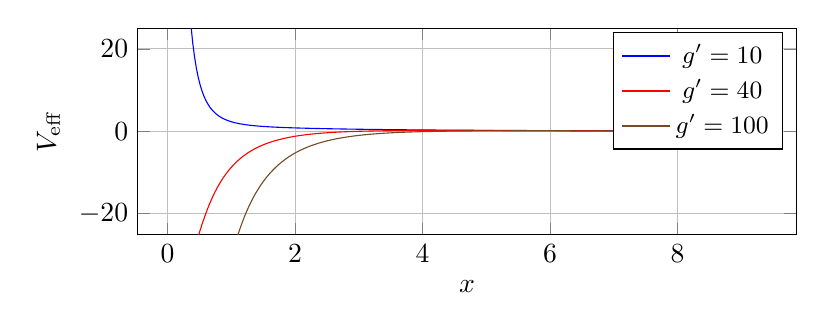
\begin{tikzpicture}
\begin{axis}[width=.82\textwidth,height=4.2cm,xlabel={$x$},ylabel={$V_{\rm eff}$},grid=major,legend style={font=\small},ymin=-25,ymax=25]
\addplot+[mark=none] coordinates{(0.25,64.8479687) (0.279166667,49.8927728) (0.308333333,39.2846127) (0.3375,31.5326164) (0.366666667,25.7269914) (0.395833333,21.2885204) (0.425,17.8351746) (0.454166667,15.1073179) (0.483333333,12.9238985) (0.5125,11.1558145) (0.541666667,9.70919065) (0.570833333,8.51457857) (0.6,7.51980607) (0.629166667,6.68513756) (0.658333333,5.97993317) (0.6875,5.38030101) (0.716666667,4.86742091) (0.745833333,4.42632967) (0.775,4.04502926) (0.804166667,3.71382385) (0.833333333,3.4248215) (0.8625,3.17155566) (0.891666667,2.94869495) (0.920833333,2.75181861) (0.95,2.5772413) (0.979166667,2.42187543) (1.00833333,2.28312203) (1.0375,2.15878389) (1.06666667,2.04699575) (1.09583333,1.946168) (1.125,1.85494103) (1.15416667,1.77214788) (1.18333333,1.69678371) (1.2125,1.62798056) (1.24166667,1.56498655) (1.27083333,1.5071485) (1.3,1.45389745) (1.32916667,1.40473661) (1.35833333,1.35923109) (1.3875,1.31699936) (1.41666667,1.27770591) (1.44583333,1.24105513) (1.475,1.20678599) (1.50416667,1.17466758) (1.53333333,1.1444952) (1.5625,1.11608712) (1.59166667,1.08928167) (1.62083333,1.06393478) (1.65,1.03991791) (1.67916667,1.01711611) (1.70833333,0.995426489) (1.7375,0.974756779) (1.76666667,0.955024125) (1.79583333,0.936154012) (1.825,0.918079338) (1.85416667,0.900739584) (1.88333333,0.884080099) (1.9125,0.868051462) (1.94166667,0.852608925) (1.97083333,0.837711911) (2,0.823323584) (2.02916667,0.809410457) (2.05833333,0.795942051) (2.0875,0.782890583) (2.11666667,0.770230703) (2.14583333,0.757939244) (2.175,0.745995013) (2.20416667,0.734378591) (2.23333333,0.723072169) (2.2625,0.712059385) (2.29166667,0.701325193) (2.32083333,0.690855738) (2.35,0.680638241) (2.37916667,0.670660904) (2.40833333,0.660912816) (2.4375,0.651383877) (2.46666667,0.64206472) (2.49583333,0.63294665) (2.525,0.624021583) (2.55416667,0.615281989) (2.58333333,0.606720852) (2.6125,0.598331616) (2.64166667,0.590108155) (2.67083333,0.582044731) (2.7,0.574135961) (2.72916667,0.566376793) (2.75833333,0.558762475) (2.7875,0.55128853) (2.81666667,0.543950737) (2.84583333,0.536745107) (2.875,0.52966787) (2.90416667,0.522715453) (2.93333333,0.515884467) (2.9625,0.509171692) (2.99166667,0.502574069) (3.02083333,0.49608868) (3.05,0.489712745) (3.07916667,0.483443607) (3.10833333,0.477278729) (3.1375,0.47121568) (3.16666667,0.465252129) (3.19583333,0.45938584) (3.225,0.453614667) (3.25416667,0.447936542) (3.28333333,0.442349478) (3.3125,0.436851557) (3.34166667,0.431440928) (3.37083333,0.426115807) (3.4,0.420874466) (3.42916667,0.415715234) (3.45833333,0.410636493) (3.4875,0.405636677) (3.51666667,0.400714263) (3.54583333,0.395867776) (3.575,0.391095782) (3.60416667,0.386396887) (3.63333333,0.381769735) (3.6625,0.377213007) (3.69166667,0.372725418) (3.72083333,0.368305715) (3.75,0.363952678) (3.77916667,0.359665116) (3.80833333,0.355441866) (3.8375,0.351281795) (3.86666667,0.347183794) (3.89583333,0.34314678) (3.925,0.339169695) (3.95416667,0.335251502) (3.98333333,0.33139119) (4.0125,0.327587768) (4.04166667,0.323840265) (4.07083333,0.320147732) (4.1,0.316509239) (4.12916667,0.312923874) (4.15833333,0.309390745) (4.1875,0.305908977) (4.21666667,0.302477712) (4.24583333,0.299096108) (4.275,0.295763341) (4.30416667,0.292478603) (4.33333333,0.289241099) (4.3625,0.286050052) (4.39166667,0.282904696) (4.42083333,0.279804283) (4.45,0.276748076) (4.47916667,0.273735353) (4.50833333,0.270765405) (4.5375,0.267837535) (4.56666667,0.26495106) (4.59583333,0.262105309) (4.625,0.259299621) (4.65416667,0.25653335) (4.68333333,0.253805858) (4.7125,0.251116522) (4.74166667,0.248464728) (4.77083333,0.245849871) (4.8,0.24327136) (4.82916667,0.240728613) (4.85833333,0.238221057) (4.8875,0.235748131) (4.91666667,0.233309281) (4.94583333,0.230903965) (4.975,0.228531651) (5.00416667,0.226191812) (5.03333333,0.223883935) (5.0625,0.221607512) (5.09166667,0.219362047) (5.12083333,0.217147049) (5.15,0.214962038) (5.17916667,0.212806542) (5.20833333,0.210680095) (5.2375,0.208582241) (5.26666667,0.206512531) (5.29583333,0.204470523) (5.325,0.202455785) (5.35416667,0.200467888) (5.38333333,0.198506415) (5.4125,0.196570953) (5.44166667,0.194661097) (5.47083333,0.192776447) (5.5,0.190916614) (5.52916667,0.189081211) (5.55833333,0.18726986) (5.5875,0.185482189) (5.61666667,0.183717832) (5.64583333,0.181976429) (5.675,0.180257627) (5.70416667,0.178561077) (5.73333333,0.176886438) (5.7625,0.175233373) (5.79166667,0.173601553) (5.82083333,0.171990651) (5.85,0.170400348) (5.87916667,0.16883033) (5.90833333,0.167280288) (5.9375,0.165749918) (5.96666667,0.164238921) (5.99583333,0.162747003) (6.025,0.161273877) (6.05416667,0.159819256) (6.08333333,0.158382863) (6.1125,0.156964422) (6.14166667,0.155563663) (6.17083333,0.154180321) (6.2,0.152814134) (6.22916667,0.151464845) (6.25833333,0.150132202) (6.2875,0.148815957) (6.31666667,0.147515864) (6.34583333,0.146231684) (6.375,0.14496318) (6.40416667,0.14371012) (6.43333333,0.142472275) (6.4625,0.141249421) (6.49166667,0.140041336) (6.52083333,0.138847803) (6.55,0.137668607) (6.57916667,0.13650354) (6.60833333,0.135352392) (6.6375,0.134214962) (6.66666667,0.133091049) (6.69583333,0.131980456) (6.725,0.130882989) (6.75416667,0.129798458) (6.78333333,0.128726675) (6.8125,0.127667457) (6.84166667,0.126620621) (6.87083333,0.125585989) (6.9,0.124563386) (6.92916667,0.123552639) (6.95833333,0.122553579) (6.9875,0.121566038) (7.01666667,0.120589851) (7.04583333,0.119624858) (7.075,0.118670899) (7.10416667,0.117727818) (7.13333333,0.11679546) (7.1625,0.115873674) (7.19166667,0.114962312) (7.22083333,0.114061225) (7.25,0.113170271) (7.27916667,0.112289306) (7.30833333,0.111418192) (7.3375,0.110556791) (7.36666667,0.109704967) (7.39583333,0.108862588) (7.425,0.108029522) (7.45416667,0.10720564) (7.48333333,0.106390816) (7.5125,0.105584925) (7.54166667,0.104787843) (7.57083333,0.10399945) (7.6,0.103219628) (7.62916667,0.102448258) (7.65833333,0.101685225) (7.6875,0.100930416) (7.71666667,0.10018372) (7.74583333,0.0994450257) (7.775,0.0987142258) (7.80416667,0.0979912135) (7.83333333,0.0972758839) (7.8625,0.096568134) (7.89166667,0.095867862) (7.92083333,0.0951749679) (7.95,0.0944893534) (7.97916667,0.0938109214) (8.00833333,0.0931395766) (8.0375,0.0924752249) (8.06666667,0.091817774) (8.09583333,0.0911671326) (8.125,0.0905232112) (8.15416667,0.0898859215) (8.18333333,0.0892551765) (8.2125,0.0886308907) (8.24166667,0.0880129797) (8.27083333,0.0874013606) (8.3,0.0867959516) (8.32916667,0.0861966722) (8.35833333,0.0856034433) (8.3875,0.0850161866) (8.41666667,0.0844348255) (8.44583333,0.0838592841) (8.475,0.0832894879) (8.50416667,0.0827253634) (8.53333333,0.0821668384) (8.5625,0.0816138416) (8.59166667,0.0810663028) (8.62083333,0.0805241528) (8.65,0.0799873237) (8.67916667,0.0794557483) (8.70833333,0.0789293606) (8.7375,0.0784080954) (8.76666667,0.0778918887) (8.79583333,0.0773806773) (8.825,0.076874399) (8.85416667,0.0763729924) (8.88333333,0.0758763971) (8.9125,0.0753845537) (8.94166667,0.0748974034) (8.97083333,0.0744148885) (9,0.0739369521)};
\addlegendentry{$g^\prime=10$}
\addplot+[mark=none] coordinates{(0.25,-28.6081253) (0.279166667,-31.3934888) (0.308333333,-32.1968303) (0.3375,-31.8942258) (0.366666667,-30.9763321) (0.395833333,-29.7268047) (0.425,-28.3132808) (0.454166667,-26.83611) (0.483333333,-25.3555355) (0.5125,-23.9073786) (0.541666667,-22.5123498) (0.570833333,-21.1817092) (0.6,-19.9207757) (0.629166667,-18.7311396) (0.658333333,-17.6120731) (0.6875,-16.5614406) (0.716666667,-15.5762872) (0.745833333,-14.653222) (0.775,-13.7886655) (0.804166667,-12.9790089) (0.833333333,-12.220714) (0.8625,-11.5103747) (0.891666667,-10.844752) (0.920833333,-10.2207921) (0.95,-9.63563312) (0.979166667,-9.08660422) (1.00833333,-8.57122063) (1.0375,-8.08717536) (1.06666667,-7.63232951) (1.09583333,-7.20470184) (1.125,-6.8024581) (1.15416667,-6.42390049) (1.18333333,-6.06745751) (1.2125,-5.7316743) (1.24166667,-5.41520355) (1.27083333,-5.11679704) (1.3,-4.83529777) (1.32916667,-4.56963269) (1.35833333,-4.318806) (1.3875,-4.08189301) (1.41666667,-3.85803449) (1.44583333,-3.64643151) (1.475,-3.44634066) (1.50416667,-3.25706975) (1.53333333,-3.07797382) (1.5625,-2.90845151) (1.59166667,-2.74794172) (1.62083333,-2.59592058) (1.65,-2.45189861) (1.67916667,-2.31541823) (1.70833333,-2.18605133) (1.7375,-2.06339719) (1.76666667,-1.94708043) (1.79583333,-1.83674925) (1.825,-1.73207372) (1.85416667,-1.63274423) (1.88333333,-1.53847011) (1.9125,-1.44897831) (1.94166667,-1.36401216) (1.97083333,-1.28333031) (2,-1.20670566) (2.02916667,-1.13392444) (2.05833333,-1.06478529) (2.0875,-0.999098502) (2.11666667,-0.936685224) (2.14583333,-0.877376777) (2.175,-0.821014003) (2.20416667,-0.767446666) (2.23333333,-0.716532889) (2.2625,-0.66813864) (2.29166667,-0.622137243) (2.32083333,-0.57840893) (2.35,-0.536840425) (2.37916667,-0.497324548) (2.40833333,-0.459759854) (2.4375,-0.424050292) (2.46666667,-0.390104889) (2.49583333,-0.357837452) (2.525,-0.327166292) (2.55416667,-0.298013963) (2.58333333,-0.27030702) (2.6125,-0.243975794) (2.64166667,-0.218954177) (2.67083333,-0.195179422) (2.7,-0.172591958) (2.72916667,-0.151135213) (2.75833333,-0.130755451) (2.7875,-0.111401612) (2.81666667,-0.0930251762) (2.84583333,-0.0755800176) (2.875,-0.0590222812) (2.90416667,-0.0433102601) (2.93333333,-0.0284042823) (2.9625,-0.014266603) (2.99166667,-0.000861304084) (3.02083333,0.0118458014) (3.05,0.0238872587) (3.07916667,0.0352940562) (3.10833333,0.046095705) (3.1375,0.0563203145) (3.16666667,0.0659946637) (3.19583333,0.0751442679) (3.225,0.0837934429) (3.25416667,0.0919653643) (3.28333333,0.0996821249) (3.3125,0.106964788) (3.34166667,0.113833439) (3.37083333,0.120307232) (3.4,0.126404436) (3.42916667,0.13214248) (3.45833333,0.13753799) (3.4875,0.142606829) (3.51666667,0.147364139) (3.54583333,0.151824365) (3.575,0.1560013) (3.60416667,0.159908106) (3.63333333,0.163557351) (3.6625,0.166961033) (3.69166667,0.170130609) (3.72083333,0.173077019) (3.75,0.175810711) (3.77916667,0.178341663) (3.80833333,0.180679407) (3.8375,0.182833046) (3.86666667,0.184811277) (3.89583333,0.18662241) (3.925,0.188274381) (3.95416667,0.189774776) (3.98333333,0.19113084) (4.0125,0.1923495) (4.04166667,0.193437371) (4.07083333,0.194400777) (4.1,0.195245761) (4.12916667,0.195978097) (4.15833333,0.196603307) (4.1875,0.197126663) (4.21666667,0.197553209) (4.24583333,0.197887763) (4.275,0.198134929) (4.30416667,0.198299111) (4.33333333,0.198384516) (4.3625,0.198395164) (4.39166667,0.198334899) (4.42083333,0.198207396) (4.45,0.198016164) (4.47916667,0.197764559) (4.50833333,0.197455788) (4.5375,0.197092917) (4.56666667,0.196678874) (4.59583333,0.196216459) (4.625,0.195708345) (4.65416667,0.195157089) (4.68333333,0.194565134) (4.7125,0.193934811) (4.74166667,0.193268351) (4.77083333,0.192567883) (4.8,0.191835441) (4.82916667,0.191072968) (4.85833333,0.19028232) (4.8875,0.189465269) (4.91666667,0.188623507) (4.94583333,0.18775865) (4.975,0.18687224) (5.00416667,0.18596575) (5.03333333,0.185040586) (5.0625,0.184098088) (5.09166667,0.183139536) (5.12083333,0.182166151) (5.15,0.181179098) (5.17916667,0.180179487) (5.20833333,0.179168378) (5.2375,0.178146781) (5.26666667,0.177115657) (5.29583333,0.176075923) (5.325,0.175028455) (5.35416667,0.173974084) (5.38333333,0.172913602) (5.4125,0.171847766) (5.44166667,0.170777292) (5.47083333,0.169702864) (5.5,0.168625133) (5.52916667,0.167544717) (5.55833333,0.166462204) (5.5875,0.165378151) (5.61666667,0.16429309) (5.64583333,0.163207524) (5.675,0.162121932) (5.70416667,0.161036767) (5.73333333,0.159952458) (5.7625,0.158869415) (5.79166667,0.157788023) (5.82083333,0.156708647) (5.85,0.155631634) (5.87916667,0.154557311) (5.90833333,0.153485987) (5.9375,0.152417953) (5.96666667,0.151353486) (5.99583333,0.150292845) (6.025,0.149236275) (6.05416667,0.148184007) (6.08333333,0.147136255) (6.1125,0.146093225) (6.14166667,0.145055106) (6.17083333,0.144022078) (6.2,0.142994308) (6.22916667,0.141971952) (6.25833333,0.140955156) (6.2875,0.139944055) (6.31666667,0.138938777) (6.34583333,0.137939438) (6.375,0.136946146) (6.40416667,0.135959001) (6.43333333,0.134978097) (6.4625,0.134003516) (6.49166667,0.133035338) (6.52083333,0.132073631) (6.55,0.13111846) (6.57916667,0.130169882) (6.60833333,0.129227949) (6.6375,0.128292708) (6.66666667,0.127364197) (6.69583333,0.126442454) (6.725,0.125527507) (6.75416667,0.124619384) (6.78333333,0.123718104) (6.8125,0.122823686) (6.84166667,0.121936142) (6.87083333,0.121055482) (6.9,0.12018171) (6.92916667,0.11931483) (6.95833333,0.11845484) (6.9875,0.117601735) (7.01666667,0.11675551) (7.04583333,0.115916153) (7.075,0.115083652) (7.10416667,0.114257991) (7.13333333,0.113439155) (7.1625,0.112627122) (7.19166667,0.111821871) (7.22083333,0.111023378) (7.25,0.110231618) (7.27916667,0.109446563) (7.30833333,0.108668184) (7.3375,0.10789645) (7.36666667,0.107131329) (7.39583333,0.106372787) (7.425,0.105620791) (7.45416667,0.104875303) (7.48333333,0.104136287) (7.5125,0.103403705) (7.54166667,0.102677516) (7.57083333,0.101957682) (7.6,0.101244161) (7.62916667,0.100536912) (7.65833333,0.099835892) (7.6875,0.0991410579) (7.71666667,0.0984523662) (7.74583333,0.0977697726) (7.775,0.0970932323) (7.80416667,0.0964227002) (7.83333333,0.0957581306) (7.8625,0.0950994775) (7.89166667,0.0944466946) (7.92083333,0.0937997353) (7.95,0.0931585528) (7.97916667,0.0925230999) (8.00833333,0.0918933295) (8.0375,0.0912691942) (8.06666667,0.0906506464) (8.09583333,0.0900376385) (8.125,0.089430123) (8.15416667,0.088828052) (8.18333333,0.088231378) (8.2125,0.0876400532) (8.24166667,0.0870540299) (8.27083333,0.0864732607) (8.3,0.085897698) (8.32916667,0.0853272944) (8.35833333,0.0847620025) (8.3875,0.0842017754) (8.41666667,0.0836465659) (8.44583333,0.0830963273) (8.475,0.0825510129) (8.50416667,0.0820105761) (8.53333333,0.0814749709) (8.5625,0.080944151) (8.59166667,0.0804180708) (8.62083333,0.0798966847) (8.65,0.0793799473) (8.67916667,0.0788678137) (8.70833333,0.0783602389) (8.7375,0.0778571786) (8.76666667,0.0773585885) (8.79583333,0.0768644246) (8.825,0.0763746433) (8.85416667,0.0758892013) (8.88333333,0.0754080556) (8.9125,0.0749311634) (8.94166667,0.0744584825) (8.97083333,0.0739899706) (9,0.0735255861)};
\addlegendentry{$g^\prime=40$}
\addplot+[mark=none] coordinates{(0.25,-215.520313) (0.279166667,-193.966012) (0.308333333,-175.159716) (0.3375,-158.74791) (0.366666667,-144.382979) (0.395833333,-131.757455) (0.425,-120.610192) (0.454166667,-110.722966) (0.483333333,-101.914403) (0.5125,-94.0337647) (0.541666667,-86.9554308) (0.570833333,-80.5742846) (0.6,-74.8019393) (0.629166667,-69.5636939) (0.658333333,-64.7960857) (0.6875,-60.4449237) (0.716666667,-56.4637033) (0.745833333,-52.8123252) (0.775,-49.456055) (0.804166667,-46.3646743) (0.833333333,-43.511785) (0.8625,-40.8742355) (0.891666667,-38.431646) (0.920833333,-36.1660137) (0.95,-34.061382) (0.979166667,-32.1035635) (1.00833333,-30.279906) (1.0375,-28.5790939) (1.06666667,-26.99098) (1.09583333,-25.5064415) (1.125,-24.1172564) (1.15416667,-22.8159972) (1.18333333,-21.5959399) (1.2125,-20.450984) (1.24166667,-19.3755838) (1.27083333,-18.3646881) (1.3,-17.4136882) (1.32916667,-16.5183713) (1.35833333,-15.6748802) (1.3875,-14.8796777) (1.41666667,-14.1295153) (1.44583333,-13.4214048) (1.475,-12.752594) (1.50416667,-12.1205444) (1.53333333,-11.5229119) (1.5625,-10.9575288) (1.59166667,-10.4223885) (1.62083333,-9.9156313) (1.65,-9.43553165) (1.67916667,-8.9804869) (1.70833333,-8.54900697) (1.7375,-8.13970512) (1.76666667,-7.75128955) (1.79583333,-7.38255578) (1.825,-7.03237982) (1.85416667,-6.69971185) (1.88333333,-6.38357054) (1.9125,-6.08303785) (1.94166667,-5.79725434) (1.97083333,-5.52541476) (2,-5.26676416) (2.02916667,-5.02059423) (2.05833333,-4.78623997) (2.0875,-4.56307667) (2.11666667,-4.35051708) (2.14583333,-4.14800882) (2.175,-3.95503204) (2.20416667,-3.77109718) (2.23333333,-3.595743) (2.2625,-3.42853469) (2.29166667,-3.26906212) (2.32083333,-3.11693827) (2.35,-2.97179776) (2.37916667,-2.83329545) (2.40833333,-2.70110519) (2.4375,-2.57491863) (2.46666667,-2.45444411) (2.49583333,-2.33940566) (2.525,-2.22954204) (2.55416667,-2.12460587) (2.58333333,-2.02436276) (2.6125,-1.92859062) (2.64166667,-1.83707884) (2.67083333,-1.74962773) (2.7,-1.6660478) (2.72916667,-1.58615923) (2.75833333,-1.5097913) (2.7875,-1.4367819) (2.81666667,-1.366977) (2.84583333,-1.30023027) (2.875,-1.23640258) (2.90416667,-1.17536169) (2.93333333,-1.11698178) (2.9625,-1.06114319) (2.99166667,-1.00773205) (3.02083333,-0.956639955) (3.05,-0.907763713) (3.07916667,-0.861005046) (3.10833333,-0.816270344) (3.1375,-0.773470416) (3.16666667,-0.732520266) (3.19583333,-0.693338877) (3.225,-0.655849005) (3.25416667,-0.619976992) (3.28333333,-0.585652581) (3.3125,-0.552808748) (3.34166667,-0.521381539) (3.37083333,-0.491309917) (3.4,-0.462535622) (3.42916667,-0.435003027) (3.45833333,-0.408659018) (3.4875,-0.383452865) (3.51666667,-0.35933611) (3.54583333,-0.336262456) (3.575,-0.314187664) (3.60416667,-0.293069455) (3.63333333,-0.272867417) (3.6625,-0.253542914) (3.69166667,-0.235059008) (3.72083333,-0.217380372) (3.75,-0.200473223) (3.77916667,-0.184305242) (3.80833333,-0.168845513) (3.8375,-0.154064454) (3.86666667,-0.139933757) (3.89583333,-0.126426332) (3.925,-0.113516246) (3.95416667,-0.101178677) (3.98333333,-0.0893898593) (4.0125,-0.0781270365) (4.04166667,-0.0673684181) (4.07083333,-0.0570931345) (4.1,-0.0472811966) (4.12916667,-0.0379134567) (4.15833333,-0.0289715709) (4.1875,-0.0204379641) (4.21666667,-0.0122957958) (4.24583333,-0.00452892809) (4.275,0.00287810527) (4.30416667,0.00994012786) (4.33333333,0.0166713487) (4.3625,0.0230853887) (4.39166667,0.0291953063) (4.42083333,0.0350136216) (4.45,0.0405523393) (4.47916667,0.0458229708) (4.50833333,0.0508365558) (4.5375,0.0556036814) (4.56666667,0.0601345023) (4.59583333,0.0644387586) (4.625,0.0685257932) (4.65416667,0.0724045691) (4.68333333,0.0760836847) (4.7125,0.0795713896) (4.74166667,0.082875599) (4.77083333,0.0860039076) (4.8,0.0889636031) (4.82916667,0.0917616789) (4.85833333,0.094404846) (4.8875,0.0968995453) (4.91666667,0.0992519583) (4.94583333,0.101468018) (4.975,0.103553418) (5.00416667,0.105513626) (5.03333333,0.107353887) (5.0625,0.109079238) (5.09166667,0.110694514) (5.12083333,0.112204355) (5.15,0.113613218) (5.17916667,0.114925379) (5.20833333,0.116144946) (5.2375,0.117275861) (5.26666667,0.118321908) (5.29583333,0.119286724) (5.325,0.120173796) (5.35416667,0.120986474) (5.38333333,0.121727977) (5.4125,0.122401391) (5.44166667,0.123009682) (5.47083333,0.123555698) (5.5,0.124042172) (5.52916667,0.12447173) (5.55833333,0.12484689) (5.5875,0.125170075) (5.61666667,0.125443606) (5.64583333,0.125669714) (5.675,0.125850542) (5.70416667,0.125988145) (5.73333333,0.126084499) (5.7625,0.126141498) (5.79166667,0.126160963) (5.82083333,0.12614464) (5.85,0.126094207) (5.87916667,0.126011273) (5.90833333,0.125897384) (5.9375,0.125754024) (5.96666667,0.125582617) (5.99583333,0.125384529) (6.025,0.125161073) (6.05416667,0.124913507) (6.08333333,0.12464304) (6.1125,0.124350831) (6.14166667,0.124037993) (6.17083333,0.123705593) (6.2,0.123354657) (6.22916667,0.122986166) (6.25833333,0.122601063) (6.2875,0.122200253) (6.31666667,0.121784603) (6.34583333,0.121354945) (6.375,0.120912077) (6.40416667,0.120456764) (6.43333333,0.11998974) (6.4625,0.119511707) (6.49166667,0.119023341) (6.52083333,0.118525287) (6.55,0.118018164) (6.57916667,0.117502567) (6.60833333,0.116979063) (6.6375,0.116448198) (6.66666667,0.115910493) (6.69583333,0.115366448) (6.725,0.114816543) (6.75416667,0.114261234) (6.78333333,0.113700962) (6.8125,0.113136144) (6.84166667,0.112567185) (6.87083333,0.111994467) (6.9,0.111418359) (6.92916667,0.110839212) (6.95833333,0.110257362) (6.9875,0.109673131) (7.01666667,0.109086827) (7.04583333,0.108498742) (7.075,0.107909156) (7.10416667,0.107318339) (7.13333333,0.106726545) (7.1625,0.106134018) (7.19166667,0.10554099) (7.22083333,0.104947685) (7.25,0.104354313) (7.27916667,0.103761076) (7.30833333,0.103168166) (7.3375,0.102575767) (7.36666667,0.101984052) (7.39583333,0.101393187) (7.425,0.100803329) (7.45416667,0.10021463) (7.48333333,0.0996272296) (7.5125,0.0990412646) (7.54166667,0.0984568629) (7.57083333,0.0978741459) (7.6,0.0972932291) (7.62916667,0.0967142214) (7.65833333,0.0961372263) (7.6875,0.0955623415) (7.71666667,0.0949896591) (7.74583333,0.0944192664) (7.775,0.0938512454) (7.80416667,0.0932856736) (7.83333333,0.0927226238) (7.8625,0.0921621645) (7.89166667,0.0916043598) (7.92083333,0.09104927) (7.95,0.0904969515) (7.97916667,0.089947457) (8.00833333,0.0894008355) (8.0375,0.0888571328) (8.06666667,0.0883163913) (8.09583333,0.0877786504) (8.125,0.0872439465) (8.15416667,0.0867123131) (8.18333333,0.0861837809) (8.2125,0.0856583781) (8.24166667,0.0851361304) (8.27083333,0.084617061) (8.3,0.0841011908) (8.32916667,0.0835885386) (8.35833333,0.0830791211) (8.3875,0.0825729529) (8.41666667,0.0820700469) (8.44583333,0.0815704138) (8.475,0.0810740628) (8.50416667,0.0805810015) (8.53333333,0.0800912358) (8.5625,0.0796047699) (8.59166667,0.079121607) (8.62083333,0.0786417485) (8.65,0.0781651946) (8.67916667,0.0776919444) (8.70833333,0.0772219957) (8.7375,0.076755345) (8.76666667,0.0762919879) (8.79583333,0.0758319191) (8.825,0.0753751319) (8.85416667,0.0749216192) (8.88333333,0.0744713726) (8.9125,0.074024383) (8.94166667,0.0735806406) (8.97083333,0.0731401347) (9,0.072702854)};
\addlegendentry{$g^\prime=100$}
\end{axis}\end{tikzpicture}\end{center}
\begin{center}\begin{tikzpicture}
\begin{axis}[width=.82\textwidth,height=4.2cm,xlabel={$x$},ylabel={$u_2$},grid=major,legend style={font=\small},legend pos=north east]
\addplot+[mark=none] coordinates{(0,0) (0.0333333333,2.76284926e-05) (0.0666666667,0.000210158363) (0.1,0.000674203238) (0.133333333,0.00151860118) (0.166666667,0.00281755207) (0.2,0.00462349377) (0.233333333,0.00696973511) (0.266666667,0.00987286287) (0.3,0.0133349387) (0.333333333,0.0173455006) (0.366666667,0.0218833843) (0.4,0.0269183754) (0.433333333,0.0324127069) (0.466666667,0.0383224126) (0.5,0.0445985472) (0.533333333,0.0511882831) (0.566666667,0.0580358935) (0.6,0.0650836317) (0.633333333,0.072272512) (0.666666667,0.0795430035) (0.7,0.0868356413) (0.733333333,0.0940915626) (0.766666667,0.101252975) (0.8,0.10826356) (0.833333333,0.115068821) (0.866666667,0.12161638) (0.9,0.12785622) (0.933333333,0.133740893) (0.966666667,0.139225681) (1,0.144268727) (1.03333333,0.148831129) (1.06666667,0.15287701) (1.1,0.156373557) (1.13333333,0.15929104) (1.16666667,0.16160281) (1.2,0.163285277) (1.23333333,0.164317875) (1.26666667,0.164683007) (1.3,0.164365987) (1.33333333,0.163354959) (1.36666667,0.161640819) (1.4,0.15921712) (1.43333333,0.156079977) (1.46666667,0.152227962) (1.5,0.147661998) (1.53333333,0.142385245) (1.56666667,0.136402993) (1.6,0.129722542) (1.63333333,0.122353088) (1.66666667,0.114305608) (1.7,0.105592745) (1.73333333,0.096228691) (1.76666667,0.0862290748) (1.8,0.0756108507) (1.83333333,0.0643921884) (1.86666667,0.0525923651) (1.9,0.0402316615) (1.93333333,0.0273312592) (1.96666667,0.0139131419) (2,0) (2.03333333,-0.0143848627) (2.06666667,-0.0292176174) (2.1,-0.0444739961) (2.13333333,-0.0601293738) (2.16666667,-0.0761588467) (2.2,-0.0925373075) (2.23333333,-0.109239516) (2.26666667,-0.126240167) (2.3,-0.143513956) (2.33333333,-0.161035635) (2.36666667,-0.178780077) (2.4,-0.196722322) (2.43333333,-0.214837631) (2.46666667,-0.233101536) (2.5,-0.251489876) (2.53333333,-0.269978844) (2.56666667,-0.288545024) (2.6,-0.30716542) (2.63333333,-0.325817496) (2.66666667,-0.344479197) (2.7,-0.363128982) (2.73333333,-0.381745843) (2.76666667,-0.400309327) (2.8,-0.418799556) (2.83333333,-0.437197244) (2.86666667,-0.45548371) (2.9,-0.473640888) (2.93333333,-0.491651343) (2.96666667,-0.509498274) (3,-0.527165523) (3.03333333,-0.54463758) (3.06666667,-0.561899585) (3.1,-0.57893733) (3.13333333,-0.59573726) (3.16666667,-0.61228647) (3.2,-0.628572707) (3.23333333,-0.644584361) (3.26666667,-0.660310462) (3.3,-0.675740677) (3.33333333,-0.690865301) (3.36666667,-0.705675248) (3.4,-0.720162046) (3.43333333,-0.734317825) (3.46666667,-0.74813531) (3.5,-0.761607806) (3.53333333,-0.774729191) (3.56666667,-0.787493905) (3.6,-0.799896932) (3.63333333,-0.811933795) (3.66666667,-0.823600538) (3.7,-0.834893715) (3.73333333,-0.845810375) (3.76666667,-0.856348051) (3.8,-0.866504744) (3.83333333,-0.876278909) (3.86666667,-0.885669441) (3.9,-0.894675663) (3.93333333,-0.903297307) (3.96666667,-0.911534505) (4,-0.919387772) (4.03333333,-0.926857989) (4.06666667,-0.933946396) (4.1,-0.940654571) (4.13333333,-0.946984418) (4.16666667,-0.952938156) (4.2,-0.9585183) (4.23333333,-0.963727654) (4.26666667,-0.968569289) (4.3,-0.973046538) (4.33333333,-0.977162977) (4.36666667,-0.980922418) (4.4,-0.98432889) (4.43333333,-0.98738663) (4.46666667,-0.99010007) (4.5,-0.992473827) (4.53333333,-0.994512688) (4.56666667,-0.996221602) (4.6,-0.997605666) (4.63333333,-0.998670117) (4.66666667,-0.999420317) (4.7,-0.999861749) (4.73333333,-1) (4.76666667,-0.999840758) (4.8,-0.999389797) (4.83333333,-0.998652972) (4.86666667,-0.997636206) (4.9,-0.996345486) (4.93333333,-0.994786852) (4.96666667,-0.992966387) (5,-0.990890214) (5.03333333,-0.988564485) (5.06666667,-0.985995376) (5.1,-0.983189078) (5.13333333,-0.980151791) (5.16666667,-0.976889718) (5.2,-0.973409061) (5.23333333,-0.969716008) (5.26666667,-0.965816737) (5.3,-0.961717404) (5.33333333,-0.95742414) (5.36666667,-0.952943044) (5.4,-0.948280184) (5.43333333,-0.943441585) (5.46666667,-0.93843323) (5.5,-0.933261056) (5.53333333,-0.927930946) (5.56666667,-0.92244873) (5.6,-0.91682018) (5.63333333,-0.911051007) (5.66666667,-0.905146856) (5.7,-0.899113307) (5.73333333,-0.892955869) (5.76666667,-0.88667998) (5.8,-0.880291003) (5.83333333,-0.873794226) (5.86666667,-0.867194858) (5.9,-0.860498029) (5.93333333,-0.853708785) (5.96666667,-0.846832092) (6,-0.83987283) (6.03333333,-0.832835795) (6.06666667,-0.825725696) (6.1,-0.818547155) (6.13333333,-0.811304704) (6.16666667,-0.804002789) (6.2,-0.796645766) (6.23333333,-0.7892379) (6.26666667,-0.781783367) (6.3,-0.774286254) (6.33333333,-0.766750554) (6.36666667,-0.759180174) (6.4,-0.751578928) (6.43333333,-0.74395054) (6.46666667,-0.736298644) (6.5,-0.728626785) (6.53333333,-0.720938418) (6.56666667,-0.71323691) (6.6,-0.705525538) (6.63333333,-0.697807493) (6.66666667,-0.690085876) (6.7,-0.682363705) (6.73333333,-0.674643909) (6.76666667,-0.666929333) (6.8,-0.659222739) (6.83333333,-0.651526805) (6.86666667,-0.643844124) (6.9,-0.636177211) (6.93333333,-0.628528499) (6.96666667,-0.620900341) (7,-0.613295011) (7.03333333,-0.605714708) (7.06666667,-0.598161551) (7.1,-0.590637588) (7.13333333,-0.583144789) (7.16666667,-0.575685052) (7.2,-0.568260206) (7.23333333,-0.560872005) (7.26666667,-0.553522138) (7.3,-0.546212221) (7.33333333,-0.538943808) (7.36666667,-0.531718384) (7.4,-0.524537369) (7.43333333,-0.517402124) (7.46666667,-0.510313942) (7.5,-0.50327406) (7.53333333,-0.496283653) (7.56666667,-0.489343839) (7.6,-0.482455678) (7.63333333,-0.475620175) (7.66666667,-0.46883828) (7.7,-0.462110888) (7.73333333,-0.455438846) (7.76666667,-0.448822946) (7.8,-0.442263933) (7.83333333,-0.435762502) (7.86666667,-0.429319302) (7.9,-0.422934935) (7.93333333,-0.416609957) (7.96666667,-0.410344884) (8,-0.404140186) (8.03333333,-0.397996293) (8.06666667,-0.391913594) (8.1,-0.385892439) (8.13333333,-0.379933141) (8.16666667,-0.374035975) (8.2,-0.36820118) (8.23333333,-0.362428961) (8.26666667,-0.356719489) (8.3,-0.351072901) (8.33333333,-0.345489304) (8.36666667,-0.339968774) (8.4,-0.334511356) (8.43333333,-0.329117067) (8.46666667,-0.323785897) (8.5,-0.318517808) (8.53333333,-0.313312737) (8.56666667,-0.308170595) (8.6,-0.303091269) (8.63333333,-0.298074623) (8.66666667,-0.293120499) (8.7,-0.288228717) (8.73333333,-0.283399076) (8.76666667,-0.278631355) (8.8,-0.273925315) (8.83333333,-0.269280696) (8.86666667,-0.264697224) (8.9,-0.260174604) (8.93333333,-0.255712529) (8.96666667,-0.251310673) (9,-0.246968698) (9.03333333,-0.24268625) (9.06666667,-0.238462961) (9.1,-0.234298453) (9.13333333,-0.230192334) (9.16666667,-0.2261442) (9.2,-0.222153636) (9.23333333,-0.218220219) (9.26666667,-0.214343513) (9.3,-0.210523075) (9.33333333,-0.206758452) (9.36666667,-0.203049184) (9.4,-0.199394802) (9.43333333,-0.19579483) (9.46666667,-0.192248786) (9.5,-0.188756181) (9.53333333,-0.185316522) (9.56666667,-0.181929307) (9.6,-0.178594034) (9.63333333,-0.175310191) (9.66666667,-0.172077267) (9.7,-0.168894744) (9.73333333,-0.165762102) (9.76666667,-0.162678817) (9.8,-0.159644363) (9.83333333,-0.156658213) (9.86666667,-0.153719835) (9.9,-0.150828699) (9.93333333,-0.147984271) (9.96666667,-0.145186017) (10,-0.142433402)};
\addlegendentry{定性径向态}
\end{axis}\end{tikzpicture}\end{center}

\end{solution}
\originalsection{正式第6题：超精细加磁场}
\begin{exercise}
两自旋1/2, $H'=2\varepsilon S_{ez}/\hbar+4\varepsilon'\boldsymbol S_e\cdot\boldsymbol S_p/\hbar^2$, $\varepsilon=\mu_BB$, $\varepsilon'>0$. 在未耦合$(\uparrow\uparrow,\uparrow\downarrow,\downarrow\uparrow,\downarrow\downarrow)$及耦合$(1,1),(1,0),(1,-1),(0,0)$基求矩阵、本征对, 图能量随$B$, 给弱场一阶态及能量并判断两基适用性.
\end{exercise}
\begin{solution}
未耦合矩阵端格为$\varepsilon'+\varepsilon,\varepsilon'-\varepsilon$, 中块$\begin{pmatrix}\varepsilon-\varepsilon'&2\varepsilon'\\2\varepsilon'&-\varepsilon-\varepsilon'\end{pmatrix}$. 耦合基同两端, 在$(T_0,S)$中块为$\begin{pmatrix}\varepsilon'&\varepsilon\\\varepsilon&-3\varepsilon'\end{pmatrix}$. 记$D=\sqrt{\varepsilon^2+4\varepsilon'^2}$, 能量两端$\varepsilon'\pm\varepsilon$, 中间$-\varepsilon'\pm D$. 令$\theta=\frac12\arctan[\varepsilon/(2\varepsilon')]$（连续取$|\theta|<\pi/4$）, 高态$\cos\theta T_0+\sin\theta S$, 低态$-\sin\theta T_0+\cos\theta S$. 将$T_0=(\uparrow\downarrow+\downarrow\uparrow)/\sqrt2,S=(\uparrow\downarrow-\downarrow\uparrow)/\sqrt2$代回即未耦合本征矢.

弱场能量至一阶为$\varepsilon'\pm\varepsilon,\varepsilon',-3\varepsilon'$, 两混合态$T_0+\varepsilon S/(4\varepsilon')$及$S-\varepsilon T_0/(4\varepsilon')$, 此阶可不归一. 小场耦合基适合, 大$|\varepsilon|$时电子自旋分量决定能量, 未耦合基适合; 接近0的混合不是把两基任意轮换. 曲线下图按$\varepsilon'$归一, 交叉是否真实取决于本Hamilton算符守恒的总$m$, 不额外加入未给的耦合.
\begin{center}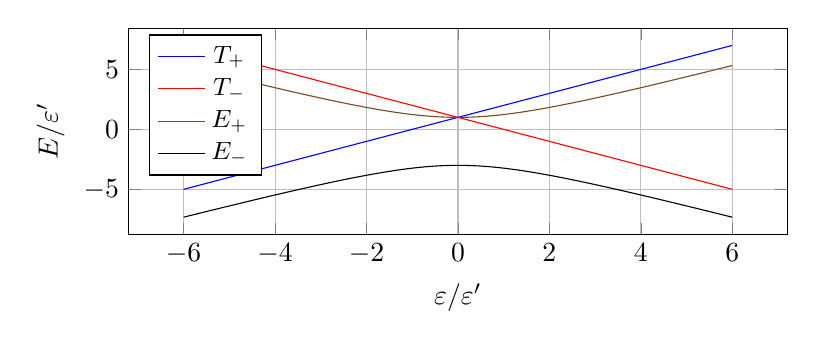
\begin{tikzpicture}
\begin{axis}[width=.82\textwidth,height=4.2cm,xlabel={$\varepsilon/\varepsilon^\prime$},ylabel={$E/\varepsilon^\prime$},grid=major,legend style={font=\small},legend pos=north west]
\addplot+[mark=none] coordinates{(-6,-5) (-5.95,-4.95) (-5.9,-4.9) (-5.85,-4.85) (-5.8,-4.8) (-5.75,-4.75) (-5.7,-4.7) (-5.65,-4.65) (-5.6,-4.6) (-5.55,-4.55) (-5.5,-4.5) (-5.45,-4.45) (-5.4,-4.4) (-5.35,-4.35) (-5.3,-4.3) (-5.25,-4.25) (-5.2,-4.2) (-5.15,-4.15) (-5.1,-4.1) (-5.05,-4.05) (-5,-4) (-4.95,-3.95) (-4.9,-3.9) (-4.85,-3.85) (-4.8,-3.8) (-4.75,-3.75) (-4.7,-3.7) (-4.65,-3.65) (-4.6,-3.6) (-4.55,-3.55) (-4.5,-3.5) (-4.45,-3.45) (-4.4,-3.4) (-4.35,-3.35) (-4.3,-3.3) (-4.25,-3.25) (-4.2,-3.2) (-4.15,-3.15) (-4.1,-3.1) (-4.05,-3.05) (-4,-3) (-3.95,-2.95) (-3.9,-2.9) (-3.85,-2.85) (-3.8,-2.8) (-3.75,-2.75) (-3.7,-2.7) (-3.65,-2.65) (-3.6,-2.6) (-3.55,-2.55) (-3.5,-2.5) (-3.45,-2.45) (-3.4,-2.4) (-3.35,-2.35) (-3.3,-2.3) (-3.25,-2.25) (-3.2,-2.2) (-3.15,-2.15) (-3.1,-2.1) (-3.05,-2.05) (-3,-2) (-2.95,-1.95) (-2.9,-1.9) (-2.85,-1.85) (-2.8,-1.8) (-2.75,-1.75) (-2.7,-1.7) (-2.65,-1.65) (-2.6,-1.6) (-2.55,-1.55) (-2.5,-1.5) (-2.45,-1.45) (-2.4,-1.4) (-2.35,-1.35) (-2.3,-1.3) (-2.25,-1.25) (-2.2,-1.2) (-2.15,-1.15) (-2.1,-1.1) (-2.05,-1.05) (-2,-1) (-1.95,-0.95) (-1.9,-0.9) (-1.85,-0.85) (-1.8,-0.8) (-1.75,-0.75) (-1.7,-0.7) (-1.65,-0.65) (-1.6,-0.6) (-1.55,-0.55) (-1.5,-0.5) (-1.45,-0.45) (-1.4,-0.4) (-1.35,-0.35) (-1.3,-0.3) (-1.25,-0.25) (-1.2,-0.2) (-1.15,-0.15) (-1.1,-0.1) (-1.05,-0.05) (-1,0) (-0.95,0.05) (-0.9,0.1) (-0.85,0.15) (-0.8,0.2) (-0.75,0.25) (-0.7,0.3) (-0.65,0.35) (-0.6,0.4) (-0.55,0.45) (-0.5,0.5) (-0.45,0.55) (-0.4,0.6) (-0.35,0.65) (-0.3,0.7) (-0.25,0.75) (-0.2,0.8) (-0.15,0.85) (-0.1,0.9) (-0.05,0.95) (0,1) (0.05,1.05) (0.1,1.1) (0.15,1.15) (0.2,1.2) (0.25,1.25) (0.3,1.3) (0.35,1.35) (0.4,1.4) (0.45,1.45) (0.5,1.5) (0.55,1.55) (0.6,1.6) (0.65,1.65) (0.7,1.7) (0.75,1.75) (0.8,1.8) (0.85,1.85) (0.9,1.9) (0.95,1.95) (1,2) (1.05,2.05) (1.1,2.1) (1.15,2.15) (1.2,2.2) (1.25,2.25) (1.3,2.3) (1.35,2.35) (1.4,2.4) (1.45,2.45) (1.5,2.5) (1.55,2.55) (1.6,2.6) (1.65,2.65) (1.7,2.7) (1.75,2.75) (1.8,2.8) (1.85,2.85) (1.9,2.9) (1.95,2.95) (2,3) (2.05,3.05) (2.1,3.1) (2.15,3.15) (2.2,3.2) (2.25,3.25) (2.3,3.3) (2.35,3.35) (2.4,3.4) (2.45,3.45) (2.5,3.5) (2.55,3.55) (2.6,3.6) (2.65,3.65) (2.7,3.7) (2.75,3.75) (2.8,3.8) (2.85,3.85) (2.9,3.9) (2.95,3.95) (3,4) (3.05,4.05) (3.1,4.1) (3.15,4.15) (3.2,4.2) (3.25,4.25) (3.3,4.3) (3.35,4.35) (3.4,4.4) (3.45,4.45) (3.5,4.5) (3.55,4.55) (3.6,4.6) (3.65,4.65) (3.7,4.7) (3.75,4.75) (3.8,4.8) (3.85,4.85) (3.9,4.9) (3.95,4.95) (4,5) (4.05,5.05) (4.1,5.1) (4.15,5.15) (4.2,5.2) (4.25,5.25) (4.3,5.3) (4.35,5.35) (4.4,5.4) (4.45,5.45) (4.5,5.5) (4.55,5.55) (4.6,5.6) (4.65,5.65) (4.7,5.7) (4.75,5.75) (4.8,5.8) (4.85,5.85) (4.9,5.9) (4.95,5.95) (5,6) (5.05,6.05) (5.1,6.1) (5.15,6.15) (5.2,6.2) (5.25,6.25) (5.3,6.3) (5.35,6.35) (5.4,6.4) (5.45,6.45) (5.5,6.5) (5.55,6.55) (5.6,6.6) (5.65,6.65) (5.7,6.7) (5.75,6.75) (5.8,6.8) (5.85,6.85) (5.9,6.9) (5.95,6.95) (6,7)};
\addlegendentry{$T_+$}
\addplot+[mark=none] coordinates{(-6,7) (-5.95,6.95) (-5.9,6.9) (-5.85,6.85) (-5.8,6.8) (-5.75,6.75) (-5.7,6.7) (-5.65,6.65) (-5.6,6.6) (-5.55,6.55) (-5.5,6.5) (-5.45,6.45) (-5.4,6.4) (-5.35,6.35) (-5.3,6.3) (-5.25,6.25) (-5.2,6.2) (-5.15,6.15) (-5.1,6.1) (-5.05,6.05) (-5,6) (-4.95,5.95) (-4.9,5.9) (-4.85,5.85) (-4.8,5.8) (-4.75,5.75) (-4.7,5.7) (-4.65,5.65) (-4.6,5.6) (-4.55,5.55) (-4.5,5.5) (-4.45,5.45) (-4.4,5.4) (-4.35,5.35) (-4.3,5.3) (-4.25,5.25) (-4.2,5.2) (-4.15,5.15) (-4.1,5.1) (-4.05,5.05) (-4,5) (-3.95,4.95) (-3.9,4.9) (-3.85,4.85) (-3.8,4.8) (-3.75,4.75) (-3.7,4.7) (-3.65,4.65) (-3.6,4.6) (-3.55,4.55) (-3.5,4.5) (-3.45,4.45) (-3.4,4.4) (-3.35,4.35) (-3.3,4.3) (-3.25,4.25) (-3.2,4.2) (-3.15,4.15) (-3.1,4.1) (-3.05,4.05) (-3,4) (-2.95,3.95) (-2.9,3.9) (-2.85,3.85) (-2.8,3.8) (-2.75,3.75) (-2.7,3.7) (-2.65,3.65) (-2.6,3.6) (-2.55,3.55) (-2.5,3.5) (-2.45,3.45) (-2.4,3.4) (-2.35,3.35) (-2.3,3.3) (-2.25,3.25) (-2.2,3.2) (-2.15,3.15) (-2.1,3.1) (-2.05,3.05) (-2,3) (-1.95,2.95) (-1.9,2.9) (-1.85,2.85) (-1.8,2.8) (-1.75,2.75) (-1.7,2.7) (-1.65,2.65) (-1.6,2.6) (-1.55,2.55) (-1.5,2.5) (-1.45,2.45) (-1.4,2.4) (-1.35,2.35) (-1.3,2.3) (-1.25,2.25) (-1.2,2.2) (-1.15,2.15) (-1.1,2.1) (-1.05,2.05) (-1,2) (-0.95,1.95) (-0.9,1.9) (-0.85,1.85) (-0.8,1.8) (-0.75,1.75) (-0.7,1.7) (-0.65,1.65) (-0.6,1.6) (-0.55,1.55) (-0.5,1.5) (-0.45,1.45) (-0.4,1.4) (-0.35,1.35) (-0.3,1.3) (-0.25,1.25) (-0.2,1.2) (-0.15,1.15) (-0.1,1.1) (-0.05,1.05) (0,1) (0.05,0.95) (0.1,0.9) (0.15,0.85) (0.2,0.8) (0.25,0.75) (0.3,0.7) (0.35,0.65) (0.4,0.6) (0.45,0.55) (0.5,0.5) (0.55,0.45) (0.6,0.4) (0.65,0.35) (0.7,0.3) (0.75,0.25) (0.8,0.2) (0.85,0.15) (0.9,0.1) (0.95,0.05) (1,0) (1.05,-0.05) (1.1,-0.1) (1.15,-0.15) (1.2,-0.2) (1.25,-0.25) (1.3,-0.3) (1.35,-0.35) (1.4,-0.4) (1.45,-0.45) (1.5,-0.5) (1.55,-0.55) (1.6,-0.6) (1.65,-0.65) (1.7,-0.7) (1.75,-0.75) (1.8,-0.8) (1.85,-0.85) (1.9,-0.9) (1.95,-0.95) (2,-1) (2.05,-1.05) (2.1,-1.1) (2.15,-1.15) (2.2,-1.2) (2.25,-1.25) (2.3,-1.3) (2.35,-1.35) (2.4,-1.4) (2.45,-1.45) (2.5,-1.5) (2.55,-1.55) (2.6,-1.6) (2.65,-1.65) (2.7,-1.7) (2.75,-1.75) (2.8,-1.8) (2.85,-1.85) (2.9,-1.9) (2.95,-1.95) (3,-2) (3.05,-2.05) (3.1,-2.1) (3.15,-2.15) (3.2,-2.2) (3.25,-2.25) (3.3,-2.3) (3.35,-2.35) (3.4,-2.4) (3.45,-2.45) (3.5,-2.5) (3.55,-2.55) (3.6,-2.6) (3.65,-2.65) (3.7,-2.7) (3.75,-2.75) (3.8,-2.8) (3.85,-2.85) (3.9,-2.9) (3.95,-2.95) (4,-3) (4.05,-3.05) (4.1,-3.1) (4.15,-3.15) (4.2,-3.2) (4.25,-3.25) (4.3,-3.3) (4.35,-3.35) (4.4,-3.4) (4.45,-3.45) (4.5,-3.5) (4.55,-3.55) (4.6,-3.6) (4.65,-3.65) (4.7,-3.7) (4.75,-3.75) (4.8,-3.8) (4.85,-3.85) (4.9,-3.9) (4.95,-3.95) (5,-4) (5.05,-4.05) (5.1,-4.1) (5.15,-4.15) (5.2,-4.2) (5.25,-4.25) (5.3,-4.3) (5.35,-4.35) (5.4,-4.4) (5.45,-4.45) (5.5,-4.5) (5.55,-4.55) (5.6,-4.6) (5.65,-4.65) (5.7,-4.7) (5.75,-4.75) (5.8,-4.8) (5.85,-4.85) (5.9,-4.9) (5.95,-4.95) (6,-5)};
\addlegendentry{$T_-$}
\addplot+[mark=none] coordinates{(-6,5.32455532) (-5.95,5.27714107) (-5.9,5.22976725) (-5.85,5.1824348) (-5.8,5.13514466) (-5.75,5.08789783) (-5.7,5.04069532) (-5.65,4.99353819) (-5.6,4.9464275) (-5.55,4.89936437) (-5.5,4.85234996) (-5.45,4.80538543) (-5.4,4.75847202) (-5.35,4.71161098) (-5.3,4.66480362) (-5.25,4.61805126) (-5.2,4.57135531) (-5.15,4.52471719) (-5.1,4.47813837) (-5.05,4.43162038) (-5,4.38516481) (-4.95,4.33877327) (-4.9,4.29244745) (-4.85,4.24618909) (-4.8,4.2) (-4.75,4.15388203) (-4.7,4.10783712) (-4.65,4.06186724) (-4.6,4.01597448) (-4.55,3.97016096) (-4.5,3.9244289) (-4.45,3.87878059) (-4.4,3.83321839) (-4.35,3.78774477) (-4.3,3.74236228) (-4.25,3.69707356) (-4.2,3.65188134) (-4.15,3.60678847) (-4.1,3.56179789) (-4.05,3.51691266) (-4,3.47213595) (-3.95,3.42747106) (-3.9,3.3829214) (-3.85,3.33849052) (-3.8,3.29418211) (-3.75,3.25) (-3.7,3.20594817) (-3.65,3.16203075) (-3.6,3.11825206) (-3.55,3.07461655) (-3.5,3.03112887) (-3.45,2.98779388) (-3.4,2.94461658) (-3.35,2.90160223) (-3.3,2.85875628) (-3.25,2.81608438) (-3.2,2.77359245) (-3.15,2.73128664) (-3.1,2.68917335) (-3.05,2.64725924) (-3,2.60555128) (-2.95,2.56405668) (-2.9,2.52278299) (-2.85,2.48173807) (-2.8,2.44093011) (-2.75,2.40036763) (-2.7,2.36005952) (-2.65,2.32001506) (-2.6,2.28024389) (-2.55,2.24075608) (-2.5,2.20156212) (-2.45,2.16267292) (-2.4,2.12409987) (-2.35,2.08585482) (-2.3,2.04795013) (-2.25,2.01039864) (-2.2,1.97321375) (-2.15,1.93640937) (-2.1,1.9) (-2.05,1.8640007) (-2,1.82842712) (-1.95,1.79329554) (-1.9,1.75862284) (-1.85,1.72442655) (-1.8,1.69072481) (-1.75,1.65753645) (-1.7,1.62488095) (-1.65,1.59277843) (-1.6,1.56124969) (-1.55,1.53031619) (-1.5,1.5) (-1.45,1.47032387) (-1.4,1.44131112) (-1.35,1.4129857) (-1.3,1.38537209) (-1.25,1.35849528) (-1.2,1.33238076) (-1.15,1.3070544) (-1.1,1.28254244) (-1.05,1.2588714) (-1,1.23606798) (-0.95,1.21415898) (-0.9,1.19317122) (-0.85,1.17313138) (-0.8,1.15406592) (-0.75,1.13600094) (-0.7,1.11896201) (-0.65,1.10297408) (-0.6,1.0880613) (-0.55,1.07424685) (-0.5,1.06155281) (-0.45,1.05) (-0.4,1.03960781) (-0.35,1.03039405) (-0.3,1.02237484) (-0.25,1.01556444) (-0.2,1.00997512) (-0.15,1.00561711) (-0.1,1.00249844) (-0.05,1.0006249) (0,1) (0.05,1.0006249) (0.1,1.00249844) (0.15,1.00561711) (0.2,1.00997512) (0.25,1.01556444) (0.3,1.02237484) (0.35,1.03039405) (0.4,1.03960781) (0.45,1.05) (0.5,1.06155281) (0.55,1.07424685) (0.6,1.0880613) (0.65,1.10297408) (0.7,1.11896201) (0.75,1.13600094) (0.8,1.15406592) (0.85,1.17313138) (0.9,1.19317122) (0.95,1.21415898) (1,1.23606798) (1.05,1.2588714) (1.1,1.28254244) (1.15,1.3070544) (1.2,1.33238076) (1.25,1.35849528) (1.3,1.38537209) (1.35,1.4129857) (1.4,1.44131112) (1.45,1.47032387) (1.5,1.5) (1.55,1.53031619) (1.6,1.56124969) (1.65,1.59277843) (1.7,1.62488095) (1.75,1.65753645) (1.8,1.69072481) (1.85,1.72442655) (1.9,1.75862284) (1.95,1.79329554) (2,1.82842712) (2.05,1.8640007) (2.1,1.9) (2.15,1.93640937) (2.2,1.97321375) (2.25,2.01039864) (2.3,2.04795013) (2.35,2.08585482) (2.4,2.12409987) (2.45,2.16267292) (2.5,2.20156212) (2.55,2.24075608) (2.6,2.28024389) (2.65,2.32001506) (2.7,2.36005952) (2.75,2.40036763) (2.8,2.44093011) (2.85,2.48173807) (2.9,2.52278299) (2.95,2.56405668) (3,2.60555128) (3.05,2.64725924) (3.1,2.68917335) (3.15,2.73128664) (3.2,2.77359245) (3.25,2.81608438) (3.3,2.85875628) (3.35,2.90160223) (3.4,2.94461658) (3.45,2.98779388) (3.5,3.03112887) (3.55,3.07461655) (3.6,3.11825206) (3.65,3.16203075) (3.7,3.20594817) (3.75,3.25) (3.8,3.29418211) (3.85,3.33849052) (3.9,3.3829214) (3.95,3.42747106) (4,3.47213595) (4.05,3.51691266) (4.1,3.56179789) (4.15,3.60678847) (4.2,3.65188134) (4.25,3.69707356) (4.3,3.74236228) (4.35,3.78774477) (4.4,3.83321839) (4.45,3.87878059) (4.5,3.9244289) (4.55,3.97016096) (4.6,4.01597448) (4.65,4.06186724) (4.7,4.10783712) (4.75,4.15388203) (4.8,4.2) (4.85,4.24618909) (4.9,4.29244745) (4.95,4.33877327) (5,4.38516481) (5.05,4.43162038) (5.1,4.47813837) (5.15,4.52471719) (5.2,4.57135531) (5.25,4.61805126) (5.3,4.66480362) (5.35,4.71161098) (5.4,4.75847202) (5.45,4.80538543) (5.5,4.85234996) (5.55,4.89936437) (5.6,4.9464275) (5.65,4.99353819) (5.7,5.04069532) (5.75,5.08789783) (5.8,5.13514466) (5.85,5.1824348) (5.9,5.22976725) (5.95,5.27714107) (6,5.32455532)};
\addlegendentry{$E_+$}
\addplot+[mark=none] coordinates{(-6,-7.32455532) (-5.95,-7.27714107) (-5.9,-7.22976725) (-5.85,-7.1824348) (-5.8,-7.13514466) (-5.75,-7.08789783) (-5.7,-7.04069532) (-5.65,-6.99353819) (-5.6,-6.9464275) (-5.55,-6.89936437) (-5.5,-6.85234996) (-5.45,-6.80538543) (-5.4,-6.75847202) (-5.35,-6.71161098) (-5.3,-6.66480362) (-5.25,-6.61805126) (-5.2,-6.57135531) (-5.15,-6.52471719) (-5.1,-6.47813837) (-5.05,-6.43162038) (-5,-6.38516481) (-4.95,-6.33877327) (-4.9,-6.29244745) (-4.85,-6.24618909) (-4.8,-6.2) (-4.75,-6.15388203) (-4.7,-6.10783712) (-4.65,-6.06186724) (-4.6,-6.01597448) (-4.55,-5.97016096) (-4.5,-5.9244289) (-4.45,-5.87878059) (-4.4,-5.83321839) (-4.35,-5.78774477) (-4.3,-5.74236228) (-4.25,-5.69707356) (-4.2,-5.65188134) (-4.15,-5.60678847) (-4.1,-5.56179789) (-4.05,-5.51691266) (-4,-5.47213595) (-3.95,-5.42747106) (-3.9,-5.3829214) (-3.85,-5.33849052) (-3.8,-5.29418211) (-3.75,-5.25) (-3.7,-5.20594817) (-3.65,-5.16203075) (-3.6,-5.11825206) (-3.55,-5.07461655) (-3.5,-5.03112887) (-3.45,-4.98779388) (-3.4,-4.94461658) (-3.35,-4.90160223) (-3.3,-4.85875628) (-3.25,-4.81608438) (-3.2,-4.77359245) (-3.15,-4.73128664) (-3.1,-4.68917335) (-3.05,-4.64725924) (-3,-4.60555128) (-2.95,-4.56405668) (-2.9,-4.52278299) (-2.85,-4.48173807) (-2.8,-4.44093011) (-2.75,-4.40036763) (-2.7,-4.36005952) (-2.65,-4.32001506) (-2.6,-4.28024389) (-2.55,-4.24075608) (-2.5,-4.20156212) (-2.45,-4.16267292) (-2.4,-4.12409987) (-2.35,-4.08585482) (-2.3,-4.04795013) (-2.25,-4.01039864) (-2.2,-3.97321375) (-2.15,-3.93640937) (-2.1,-3.9) (-2.05,-3.8640007) (-2,-3.82842712) (-1.95,-3.79329554) (-1.9,-3.75862284) (-1.85,-3.72442655) (-1.8,-3.69072481) (-1.75,-3.65753645) (-1.7,-3.62488095) (-1.65,-3.59277843) (-1.6,-3.56124969) (-1.55,-3.53031619) (-1.5,-3.5) (-1.45,-3.47032387) (-1.4,-3.44131112) (-1.35,-3.4129857) (-1.3,-3.38537209) (-1.25,-3.35849528) (-1.2,-3.33238076) (-1.15,-3.3070544) (-1.1,-3.28254244) (-1.05,-3.2588714) (-1,-3.23606798) (-0.95,-3.21415898) (-0.9,-3.19317122) (-0.85,-3.17313138) (-0.8,-3.15406592) (-0.75,-3.13600094) (-0.7,-3.11896201) (-0.65,-3.10297408) (-0.6,-3.0880613) (-0.55,-3.07424685) (-0.5,-3.06155281) (-0.45,-3.05) (-0.4,-3.03960781) (-0.35,-3.03039405) (-0.3,-3.02237484) (-0.25,-3.01556444) (-0.2,-3.00997512) (-0.15,-3.00561711) (-0.1,-3.00249844) (-0.05,-3.0006249) (0,-3) (0.05,-3.0006249) (0.1,-3.00249844) (0.15,-3.00561711) (0.2,-3.00997512) (0.25,-3.01556444) (0.3,-3.02237484) (0.35,-3.03039405) (0.4,-3.03960781) (0.45,-3.05) (0.5,-3.06155281) (0.55,-3.07424685) (0.6,-3.0880613) (0.65,-3.10297408) (0.7,-3.11896201) (0.75,-3.13600094) (0.8,-3.15406592) (0.85,-3.17313138) (0.9,-3.19317122) (0.95,-3.21415898) (1,-3.23606798) (1.05,-3.2588714) (1.1,-3.28254244) (1.15,-3.3070544) (1.2,-3.33238076) (1.25,-3.35849528) (1.3,-3.38537209) (1.35,-3.4129857) (1.4,-3.44131112) (1.45,-3.47032387) (1.5,-3.5) (1.55,-3.53031619) (1.6,-3.56124969) (1.65,-3.59277843) (1.7,-3.62488095) (1.75,-3.65753645) (1.8,-3.69072481) (1.85,-3.72442655) (1.9,-3.75862284) (1.95,-3.79329554) (2,-3.82842712) (2.05,-3.8640007) (2.1,-3.9) (2.15,-3.93640937) (2.2,-3.97321375) (2.25,-4.01039864) (2.3,-4.04795013) (2.35,-4.08585482) (2.4,-4.12409987) (2.45,-4.16267292) (2.5,-4.20156212) (2.55,-4.24075608) (2.6,-4.28024389) (2.65,-4.32001506) (2.7,-4.36005952) (2.75,-4.40036763) (2.8,-4.44093011) (2.85,-4.48173807) (2.9,-4.52278299) (2.95,-4.56405668) (3,-4.60555128) (3.05,-4.64725924) (3.1,-4.68917335) (3.15,-4.73128664) (3.2,-4.77359245) (3.25,-4.81608438) (3.3,-4.85875628) (3.35,-4.90160223) (3.4,-4.94461658) (3.45,-4.98779388) (3.5,-5.03112887) (3.55,-5.07461655) (3.6,-5.11825206) (3.65,-5.16203075) (3.7,-5.20594817) (3.75,-5.25) (3.8,-5.29418211) (3.85,-5.33849052) (3.9,-5.3829214) (3.95,-5.42747106) (4,-5.47213595) (4.05,-5.51691266) (4.1,-5.56179789) (4.15,-5.60678847) (4.2,-5.65188134) (4.25,-5.69707356) (4.3,-5.74236228) (4.35,-5.78774477) (4.4,-5.83321839) (4.45,-5.87878059) (4.5,-5.9244289) (4.55,-5.97016096) (4.6,-6.01597448) (4.65,-6.06186724) (4.7,-6.10783712) (4.75,-6.15388203) (4.8,-6.2) (4.85,-6.24618909) (4.9,-6.29244745) (4.95,-6.33877327) (5,-6.38516481) (5.05,-6.43162038) (5.1,-6.47813837) (5.15,-6.52471719) (5.2,-6.57135531) (5.25,-6.61805126) (5.3,-6.66480362) (5.35,-6.71161098) (5.4,-6.75847202) (5.45,-6.80538543) (5.5,-6.85234996) (5.55,-6.89936437) (5.6,-6.9464275) (5.65,-6.99353819) (5.7,-7.04069532) (5.75,-7.08789783) (5.8,-7.13514466) (5.85,-7.1824348) (5.9,-7.22976725) (5.95,-7.27714107) (6,-7.32455532)};
\addlegendentry{$E_-$}
\end{axis}\end{tikzpicture}\end{center}

\end{solution}
\originalsection{练习第1题：Runge--Lenz守恒的有序推导}
\begin{exercise}
$H_f=p^2/(2m)-f(r)$,$R_f=(p\times L-L\times p)/(2m)-f(r)r$. (a)求$[p^2,f(r)r]$并说明括号Hermitian. (b)求$[p\times L-L\times p,f(r)]$并用Hermitian形式写. (c)计算$[H_f,R_f]$并证明算符守恒恰要求$rf'=-f$, 解出$f$.
\end{exercise}
\begin{solution}
以下在$r>0$共同光滑定义域, 不声称完成Coulomb奇点的全部自伴域分析. 令$q=\hbar/\ii$, $h=f'/r$, $T=p\times L-L\times p$. 从$[p_j,F]=q\partial_jF$与$\partial_j(fr_i)=f\delta_{ij}+hr_ir_j$得到
\[
[p^2,fr_i]=q\big[p_if+fp_i+(p\cdot r)r_ih+hr_i(r\cdot p)\big]\equiv qB_i.
\]
前两项互为伴随, 后两项也互为伴随, 所以$B_i$Hermitian, 乘纯虚$q$使对易子反Hermitian, 与两Hermitian量的对易相容.

因为$[L_i,f]=0$, 直接展开叉积得$[T,f]=qhK$, $K=r\times L-L\times r$. 两个$\epsilon$缩并与$[L_i,r_j]$给
\[
K=2r(r\cdot p)-2r^2p-2\ii\hbar r
=r(r\cdot p)+(p\cdot r)r-r^2p-pr^2.
\]
第二式成对伴随显出Hermitian; 径向$h$与$r,L$对易, 因而$hK$也Hermitian. 这里保留$p$与$r$次序, 不能用经典三重积删去$\hbar$项.

$[p^2,T]=0$, 记$g=f+rf'$, 利用$[p\cdot r,h]=qrh'$整理$B-hK=2gp+q(f''+2f'/r)r=gp+pg$. 故$[H_f,R_f]=([T,f]-[p^2,fr])/(2m)=\ii\hbar\{g,p\}/(2m)$. $g=0$即守恒; 反向若一阶微分算符恒等为0, 它对任意测试函数的导数系数$2g$必须0, 故$(rf)'=0$, 唯一$f=c/r$, 含$c=0$. 氢$f=e^2/r$即此特例.
\end{solution}
\originalsection{练习第2题：Runge--Lenz长度的量子修正}
\begin{exercise}
本题改用无量纲$R=(p\times L-L\times p)/(2me^2)-r/r$. 核两种写法, 推$(L\times p)\cdot r=-L^2$、$\ii\hbar(p\cdot n-n\cdot p)=2\hbar^2/r$、$(L\times p)\cdot(p\times L)=-p^2L^2$, 再求$R^2$.
\end{exercise}
\begin{solution}
记$n=r/r,C=p\times L,D=L\times p$. 正则对易给$D=-C+2\ii\hbar p$, 因而$R=(C-\ii\hbar p)/(me^2)-n=(-D+\ii\hbar p)/(me^2)-n$. 第一恒等式用$\epsilon_{ijk}L_jp_kr_i$, 交换$p_kr_i$的$\delta_{ki}$与$\epsilon$缩并为0, 余下为$-L^2$. 第二式$[p_i,n_i]=-\ii\hbar\nabla\cdot n=-2\ii\hbar/r$, 所以乘$\ii\hbar$得到\emph{正}的$2\hbar^2/r$. 第三式两$\epsilon$缩并给$(L\cdot p)(p\cdot L)-p^2L^2$, 而$L\cdot p=p\cdot L=0$, 得所需式.

同理$D\cdot p=p\cdot C=0$, 所以$(-D+\ii\hbar p)\cdot(C-\ii\hbar p)=p^2(L^2+\hbar^2)$. 两交叉项用$D\cdot n=-L^2/r,n\cdot C=L^2/r$与上面的散度项, 得$(-D+\ii\hbar p)\cdot n+n\cdot(C-\ii\hbar p)=2(L^2+\hbar^2)/r$. 加$n^2=1$后
\[
R^2=1+\left[\frac{p^2}{m^2e^4}-\frac2{me^2r}\right](L^2+\hbar^2)
=1+\frac{2H}{me^4}(L^2+\hbar^2).
\]
这也补齐正文曾作为进阶输入的长恒等式; $+\hbar^2$完全来自非对易和径向单位矢散度, 不能从经典平方直接猜掉.
\end{solution}
\originalsection{练习第3题：1与1/2的六个CG态}
\begin{exercise}
对$\ell=1,s=1/2$, 从最高态及$J_-=L_-+S_-$求全部耦合态, 用正交求下一多重态并核维数. 在$j=m=1/2$求$L_z,S_z$均值. 电子$H_B=\mu_BB(L_z+2S_z)/\hbar$, 求各耦合态能量均值, 并求$j=m=1/2$的磁能测量分布.
\end{exercise}
\begin{solution}
记$\ket{m_\ell,\pm}$未耦合态. 最高$\ket{3/2,3/2}=\ket{1,+}$, 降一次除$\hbar\sqrt3$得到$\sqrt{2/3}\ket{0,+}+\ket{1,-}/\sqrt3$. 再降依次得到
\[
\ket{3/2,-1/2}=\ket{-1,+}/\sqrt3+\sqrt{2/3}\ket{0,-},\qquad
\ket{3/2,-3/2}=\ket{-1,-}.
\]
在$M=1/2$二维空间取正交向量, 选最大$m_\ell$项正的相位, 得
\[
\ket{1/2,1/2}=\sqrt{2/3}\ket{1,-}-\ket{0,+}/\sqrt3,\quad
\ket{1/2,-1/2}=\ket{0,-}/\sqrt3-\sqrt{2/3}\ket{-1,+}.
\]
降算符系数逐步核这些符号, 维数$4+2=6$, 无更低$j$. 未取得原题所谓卷末表, 以归一、正交及降算符作用独立核验代替.

目标态$\langle L_z\rangle=2\hbar/3$, $\langle S_z\rangle=-\hbar/6$. 全六态$\langle H_B\rangle=\mu_BBg_jm$, $g_{3/2}=4/3,g_{1/2}=2/3$, 从各展开的$m_\ell+2m_s$加权可验证. 目标态测量磁能0概率2/3（$\ket{1,-}$）, $\mu_BB$概率1/3（$\ket{0,+}$）, 均值$\mu_BB/3$. 均值不代表耦合态是纯$H_B$能量本征态.
\end{solution}
\originalsection{练习第4题：一般j的最高两组}
\begin{exercise}
两粒子各角动量$j$, 求总$J=2j$及$2j-1$两多重态的最高、次高$M$归一态; 判定交换对称性并解释整组是否一致.
\end{exercise}
\begin{solution}
用$\ket{m_1,m_2}$记未耦合态,$\ket{2j,2j}=\ket{j,j}$, $J_-$一次给$\ket{2j,2j-1}=(\ket{j,j-1}+\ket{j-1,j})/\sqrt2$. 正交的次组最高态$\ket{2j-1,2j-1}=(\ket{j,j-1}-\ket{j-1,j})/\sqrt2$. 再降一次,$\ket{j-1,j-1}$贡献消去, $\ket{2j-1,2j-2}=(\ket{j,j-2}-\ket{j-2,j})/\sqrt2$, 此式要求$j\ge1$. $j=1/2$时次组$J=0$仅一态, 无次高态; $j=0$无次组. 第一组对称、第二组反对称, 交换与$J_-$对易使各组全部保持同交换性, 不只最高态如此.
\end{solution}
\originalsection{练习第5题：一般轨道与自旋1/2}
\begin{exercise}
不靠重复升降, 用$J^2$求$\ket{j=\ell+1/2,m=M+1/2}$在未耦合基的展开, $-\ell-1\le M\le\ell$, 核两端.
\end{exercise}
\begin{solution}
固定$m=M+1/2$的两基是$\ket{M,+}$和$\ket{M+1,-}$. 因$J^2=L^2+S^2+2L_zS_z+L_+S_-+L_-S_+$, 在此块$J^2/\hbar^2$为
\[
\begin{pmatrix}\ell(\ell+1)+3/4+M&\sqrt{(\ell-M)(\ell+M+1)}\\
\sqrt{(\ell-M)(\ell+M+1)}&\ell(\ell+1)+3/4-(M+1)\end{pmatrix}.
\]
对本征值$(\ell+1/2)(\ell+3/2)$解两元比例并归一, 得
\[
\ket{\ell+1/2,M+1/2}=\sqrt{\frac{\ell+M+1}{2\ell+1}}\ket{M,+}
+\sqrt{\frac{\ell-M}{2\ell+1}}\ket{M+1,-}.
\]
$M=\ell$只第一项$\ket{\ell,+}$; $M=-\ell-1$只第二项$\ket{-\ell,-}$, 零系数对应的越界基不实际使用. 相位与上一练习最高组一致. 从固定$m$二阶矩阵求解避免对任意$M$长串降算符.
\end{solution}
\originalsection{练习第6题：三个自旋1的三角形}
\begin{exercise}
三可区分spin1, $H=\Delta(S_1\cdot S_2+S_2\cdot S_3+S_3\cdot S_1)/\hbar^2$, $\Delta>0$. 求空间维数、总自旋形式、全部能量与总简并. 在$M=0$七候选态中求唯一基态, 说明$\ket{000}$系数为何0.
\end{exercise}
\begin{solution}
维数$3^3=27$, $H=\Delta(S^2/\hbar^2-6)/2$. 先$1\otimes1=0\oplus1\oplus2$, 各自再与1合成得$0\oplus3(1)\oplus2(2)\oplus3$. 总$S=0,1,2,3$能量分别$-3\Delta,-2\Delta,0,3\Delta$, 总简并$1,9,10,7$, 和27; 多重态重复数与$2S+1$都要计入.

令基态七候选系数为$a\ket{+0-}+b\ket{+-0}+c\ket{0+-}+d\ket{0-+}+e\ket{-+0}+f\ket{-0+}+g\ket{000}$. $S_+$杀死总$S=0$态, 六输出系数给$a+c=b+d=e+f=0$及$a+b+g=c+e+g=d+f+g=0$. 解得$b=-a,c=-a,d=a,e=a,f=-a,g=0$. 归一化取$a=1/\sqrt6$, 所以
\[
\ket G=\frac{\ket{+0-}-\ket{+-0}-\ket{0+-}+\ket{0-+}+\ket{-+0}-\ket{-0+}}{\sqrt6}.
\]
$S_z\ket G=S_+\ket G=0$, 用$S^2=S_-S_++S_z^2+\hbar S_z$确证$S=0$. 只知$M=0$本身不足以断言基态.
\end{solution}
